\chapter{Drift-reduced models for plasma turbulence}
\label{chap:ModellingEdgePlasmaTurbulence}

The mechanisms at play at the plasma boundary result from the complex interplay of transport processes in the plasma, losses at the wall, and complex atomic and molecular interactions. In this region, particles experience very fast transport along the magnetic field lines and slower, often turbulence-driven, anomalous cross-field transport \cite{loarte2007}. The ratio between these phenomena characterizes the decay length of density and temperature profiles, which further determine the confinement quality of the core plasma and the total heat exhaust on the divertor target. \\

The difficulty in obtaining global experimental measurements in tokamaks requires complementary numerical simulations. Currently, these numerical data are essential to complement experimental measurements and support their interpretation. In the longer term, they will be used to make predictions and support the design of ITER experiments. Self-consistent simulations of the plasma edge are challenged by a complex geometry and the variety of involved scales. The magnetic equilibrium exhibits both open and closed magnetic field lines, breaking the toroidal symmetry. Turbulent fluctuations typically have sizes on the order of the ion gyroradius $\rho_\alpha$ ($\ge 0.4\, \text{mm}$) \cite{hennequin2004} in the perpendicular direction to the magnetic field lines, and compete with phenomena occurring along them on the order of the parallel connection length $\propto q_s R_0$ (where $q_s$ is the safety factor, and $R_0$ the tokamak major radius), which can extend up to 100 meters. \\


In this context, kinetic models based on the particle distribution function \cite{DifPradalier_2009, Charidakos_2018} are still limited to fundamental studies because of their very high numerical cost in a (5) 6-dimensional phase space. Thus, when realistic configurations are considered, reduced-dimension (2D/3D) fluid models remain the only feasible option for studying transport and turbulence at the edge of the plasma, although they are only rigorously valid in collisional regimes. A wide range of models have been derived in the literature and implemented in state-of-the-art codes \cite{DUDSON_2009, giacomin2022gbs, stegmeir2019} (see also an exhaustive presentation in the recent review by Schwander et al. \cite{SCHWANDER_2024}). The basic assumption they share is that the turbulence is characteristically low frequency and long wavelength in nature, leading to a strong scale separation between the parallel and perpendicular directions to the magnetic field. Therefore, the plasma fluid motion perpendicular to the magnetic field can be described explicitly by the so-called velocity drifts given by the quasi-static balance between Lorentz force, pressure gradient, and electromotive force due to magnetic and electric field inhomogeneities. \\

Sec. \ref{sec:edge_driftWaves} introduces the origin of drift waves, main driver for plasma turbulence, and the drift-ordering approximation that typically applied in edge plasma. 

\section{Drift wave turbulence}
\label{sec:edge_driftWaves}

\subsection{Plasma drifts}
\label{ssec:edge_plasmaDrifts}

Plasma drifts refer to the movement of charged particles under the influence of electric and magnetic fields. These drifts do not account for the primary motion along the guiding center, as described in Section \ref{ssec:intro_magneticConfinement}. To study drift velocities, it is convenient to decompose every vector quantity into an average parallel component and a fluctuating perpendicular component, such that $\mathbf{X} = X_\parallel\mathbf{b} + \mathbf{X_\perp}$. We then express the Lorentz force equation as:

\begin{equation}
	\label{eq:edge_LorentzEquationDecomposition}
	m\partial_t\left(v_\parallel\mathbf{b} + \mathbf{v}_\perp\right) = q\left[E_\parallel\mathbf{b} + \mathbf{E}_\perp + \left(v_\parallel\mathbf{b} + \mathbf{v}_\perp\right) \times \mathbf{B}\right]
\end{equation}

Focusing on the particle's acceleration in the perpendicular direction, we derive the equation of motion:

\begin{equation}
	\label{eq:edge_EcrossBdrift}
	m\partial_t \mathbf{v}_\perp = q\left[\mathbf{E} + \left(\mathbf{v}_\perp \times \mathbf{B}\right)\right]
\end{equation}

In steady-state conditions, the electric force compensates the Lorentz force, leading to the electric drift $\mathbf{v}_E$, commonly referred to as the "E cross B" or simply "ExB" drift:

\begin{equation}
	\mathbf{v}_E = \frac{\mathbf{E}_\perp \times \mathbf{B}}{B^2}
\end{equation}

This velocity applies uniformly to all particles at all times, as it depends only on the electric and magnetic fields in place. Since neither the mass nor the charge contributes to $\mathbf{v}_E$, both electrons and ions move in the same direction at the same speed, and under the quasi-neutrality assumption, no current is generated.

For the next drift, we consider the gyromotion of a particle in a non-uniform magnetic field. Under the adiabatic condition from Eq. \ref{eq:intro_adiabaticCondition}, the magnetic moment $\mu$ of the gyrating particle is conserved along its trajectory:

\begin{equation}
	\mu = \frac{m\norm{\mathbf{v}_\perp}^2}{2B}
\end{equation}

This moment leads to a potential $U = -\mu B$, which exerts a force on the particle:

\begin{equation}
	F_{\nabla B} = -\nabla U = \frac{mv_\perp^2}{2B}\nabla B
\end{equation}

This force acts in the direction of the gradient $\nabla B$, where the magnetic field strength is lower, allowing the particle to reduce its potential energy. This results in the "grad B" drift:

\begin{equation}
	\mathbf{v}_{\nabla B} = \frac{mv_\perp^2}{2q} \frac{\mathbf{B} \times \nabla B}{B^3}
\end{equation}

The helical configuration of a tokamak causes magnetic field lines to bend. To follow the direction of $\mathbf{B}$, the particle's trajectory is curved, and a centripetal force is exerted on the particle. With the curvature radius $\mathbf{R}_c = \mathbf{b} \cdot \nabla \mathbf{b}$, the force is given by:

\begin{equation}
	\mathbf{F}_c = \frac{mv_\parallel^2}{R_c}\mathbf{R}_c = -mv_\parallel^2\frac{\mathbf{B} \cdot \nabla \mathbf{B}}{B^2}
\end{equation}

This force induces the "curvature" drift $\mathbf{v}_c$:

\begin{equation}
	\mathbf{v}_c = \frac{mv_\parallel^2}{q}\frac{\mathbf{B} \times (\mathbf{B} \cdot \nabla \mathbf{B})}{B^4}
\end{equation}

The polarization drift occurs if the electric field in the plasma varies with time. 

\begin{equation}
	\mathbf{v}_p = \frac{m}{qB^2}\frac{d\mathbf{E}}{dt}
\end{equation}

Note that the directions of "grad B", curvature or polarization drifts depend on the particle's charge, causing electrons and ions to move in opposite directions and generating an effective current. The total perpendicular velocity acting on a confined particle is the sum of all these drifts:

\begin{equation}
	\mathbf{v}_d = \mathbf{v}_E + \mathbf{v}_{\nabla B} + \mathbf{v}_c + \mathbf{v}_p
\end{equation}

In fact, any force perpendicular to the magnetic field will cause a drift:

\begin{equation}
	\mathbf{v}_F = \frac{\mathbf{B}\cross\mathbf{F}_\perp}{qB^2}
\end{equation}

All other eventual forces, such as magnetic or gravitational forces, play a subordinate role in the plasma edge and are usually not considered in fluid models. Drift velocities are always orientated in perpendicular direction to then magnetic fields. They do not interfere with (the averaged) parallel fluxes, at a magnitude of $v_{th}$, and are primarily responsible for cross-field fluxes.


\subsection{Drift-ordering approximation}
\label{ssec:edge_driftOrdering}

We focus on low-$\beta$ collisional plasmas, typically found in the edge region of a tokamak. In such plasmas, we can define a characteristic length scale $L_\parallel$ for parallel phenomena, which is on the order of the machine size (e.g., the major radius $R$), where gradients in plasma fields such as density, temperature, or magnetic field strength are established. The perpendicular scale $L_\perp$ is characteristic of cross-field structures. These scales define the parallel and perpendicular wave numbers $k_\parallel$ and $k_\perp$. In the drift ordering, the following relationships hold\cite{simakov_2003}:

\begin{align}
	\beta = \frac{2\mu_0(p_e + p_i)}{B^2} &\ll 1 & \frac{\rho_L}{L_\perp} \sim \frac{\lambda_c}{L_\parallel} &\ll 1
\end{align}

where $\rho_L$ is the ion Larmor radius, and $\lambda_c$ is the mean free path between collisions. The electric force is much weaker than the magnetic force. Similarly, characteristic plasma frequencies should be much lower than the ion cyclotron frequency, giving rise to the following ordering parameters:

\begin{align}
	\epsilon_E &= \frac{mE}{qB^2} \ll 1 & \epsilon_l &= \frac{L_\perp}{L_\parallel} \ll 1 & \epsilon_t &= \frac{\omega_\perp}{\omega_L} \ll 1
\end{align}

The averaged gyromotion of particles is parallel to the magnetic field lines, with parallel velocities $v_\parallel \approx \sqrt{2T/m}$ consistent with the kinetic energy in the plasma. Drift velocities, on the other hand, are typically much slower. Since $\nabla B$ and the curvature radius $R_c$ occur at machine scales $L_\parallel$, we can provide orders of magnitude for the three drifts introduced earlier:

\begin{align}
	v_E \sim& \epsilon_E v_\parallel & v_{\nabla B} \sim& \epsilon_l v_\parallel & v_c \sim& \epsilon_l v_\parallel & v_p \sim& \epsilon_t v_\parallel
\end{align}

This leads to the assumption in the Lorentz equation \ref{eq:edge_LorentzEquationDecomposition} that the perpendicular acceleration is negligible compared to parallel dynamics, such that $m\partial_t v_\perp \approx 0$. The perpendicular direction is assumed to always be in force equilibrium, allowing us to equate the terms $\mathbf{v} \times \mathbf{B}$ and $\mathbf{E}_\perp$. Consequently, the polarization drift can be rewritten as:

\begin{equation}
	\mathbf{v}_p = \frac{m}{qB^2}\mathbf{B} \times \frac{d\mathbf{v}}{dt}
\end{equation}

Unlike other drifts, the polarization drift depends on the variation of the total velocity. To still obtain an expression for $\mathbf{v}_\perp$, we compute it in two steps, first considering the zeroth-order and then the first-order drifts:

\begin{align}
	\mathbf{v}_\perp^{(0)} &= \mathbf{v}_E + \mathbf{v}{\nabla B} + \mathbf{v}_c \\
	\mathbf{v}_\perp^{(1)} &= \mathbf{v}_\perp^{(0)} + \frac{m}{qB^2}\mathbf{B} \times \left(\partial_t + \left(v_\parallel\mathbf{b} + \mathbf{v}_\perp^{(1)}\right) \cdot \nabla\right)\mathbf{v}_\perp^{(0)} \label{eq:edge_vPerpDrifts}
\end{align}

In the first order, the evolution of the perpendicular electric field derives from the evolution of the potential gradient $d\mathbf{E}_\perp / dt = -d\nabla_\perp \Phi / dt$. The full electric field is given by:

\begin{align}
	\mathbf{E}_\perp &= -\nabla_\perp \Phi &
	E_\parallel &= -\nabla_\parallel \Phi - \partial_t A_\parallel
\end{align}

where the time variation $\partial_t A_\parallel$ accounts for magnetic induction effects.





For the perpendicular velocity, the momentum conservation equation requires several algebraic transformations:

\begin{align}
	\mathbf{b}\cross\left[\partial_t \left(mn\mathbf{u}\right) + \grad\cdot\left(mn\mathbf{u}\otimes\mathbf{u}\right)\right] =& -\mathbf{b}\cross\grad p_\perp - \mathbf{b}\cross\grad\cdot\bar{\bar{\Pi}} + nq\mathbf{b}\cross\mathbf{E} \nonumber\\ & \qquad + nq\left(\mathbf{b}\cross\mathbf{u}\cross\mathbf{B}\right) + \mathbf{b}\cross\mathbf{R} + \mathbf{b}\cross\mathbf{S}_u \nonumber \\
	\Leftrightarrow\qquad \qquad \qquad
	\mathbf{u}_\perp =& \frac{\mathbf{b}\cross\grad p}{qnB} + \frac{\mathbf{b}\cross\grad\cdot\bar{\bar{\Pi}}}{qnB} +  \frac{\mathbf{E}\cross\mathbf{b}}{B} - \frac{\mathbf{b}\cross\left(R+S\right)}{qnB} \nonumber\\ & \qquad + \frac{\mathbf{b}}{qnB} \cross \left(\partial_t \left(mn\mathbf{u}\right) + \grad\cdot\left(mn\mathbf{u}\otimes\mathbf{u}\right)\right)
\end{align}

The expression for the perpendicular velocity $\mathbf{u}_\perp$ is not explicit as the right-hand side depends on the full velocity vector. However, we can fairly well approximate it with two calculation steps. All terms that do not depend on $u$ are first evaluated to get $\mathbf{u}_\perp^{(0)}$ (and with equation \ref{eq:RelationPerpParallelVelocity} we can also calculate $\mathbf{u}^{(0)}$), and then $\mathbf{u}_\perp^{(1)}$ is calculated by replacing every occurrence of $\mathbf{u}$ by $\mathbf{u}^{(0)}$. The terms $\mathbf{u}^*$, $\mathbf{u}_E$, $\mathbf{u}_{\perp,\Pi}$, $\mathbf{u}_{\perp,S}$ and $\mathbf{u}_{p}$ are respectively called diamagnetic, "E cross B", parallel viscous stress, friction force and polarization drifts.

\begin{align}
	\mathbf{u}_\perp^{(0)} =& \frac{\mathbf{b}\cross\grad p}{qnB} + \frac{\mathbf{E}\cross\mathbf{b}}{B} = \mathbf{u}^* + \mathbf{u}_E \label{eq:VelPerp0Component} \\	
	\mathbf{u}_\perp^{(1)} =& \frac{\mathbf{b}\cross\grad\cdot\bar{\bar{\Pi}}(\mathbf{u}^{(0)})}{qnB} - \frac{\mathbf{b}\cross\left(R(\mathbf{u}^{(0)})+S(\mathbf{u}^{(0)})\right)}{qnB} \nonumber\\ & \qquad + \frac{\mathbf{b}}{n\omega_c} \cross \left(\partial_t \left(n\mathbf{u}^{(0)}\right) + \grad\cdot\left(n\mathbf{u}^{(0)}\otimes\mathbf{u}^{(0)}\right)\right) \nonumber \\
	=& \mathbf{u}_{\perp,\Pi} + \mathbf{u}_{\perp,S} + \mathbf{u}_{p} \label{eq:VelPerp1Component} \\
	\mathbf{u}_\perp \approx& \mathbf{u}_\perp^{(0)} + \mathbf{u}_\perp^{(1)}
\end{align}

This simplification holds because the contribution of $\mathbf{u}_\perp^{(1)}$ is small, of the order of $\tau_c / \tau_{ad}$ or $\tau_c / \tau_{coll}$. Next, let us extract the divergence free contribution from the diamagnetic flux $n\mathbf{u}^*$.

\begin{align}
	\label{eq:definitionDiamagneticDrift}
	n\mathbf{u}^* =& -\grad \cross \frac{p_\perp\mathbf{B}}{qB^2} + n\tilde{u}^* \nonumber\\
	& \quad\text{with: } \tilde{u}^* = \frac{2T_\perp\mathbf{B}\cross\grad B}{qB^3} + \frac{T_\perp}{qB^2}\grad\cross\mathbf{B}
\end{align}

The second term in $\tilde{u}^*$ is usually very small and can be neglected if magnetic fields do not fluctuate. \\
The last term $u_{p}$ in \autoref{eq:VelPerp1Component} is called the polarization drift. A simple expression for the associated flux can be found through algebraic manipulations and neglecting some small curvature terms.

\begin{align}
	n\mathbf{u}_{p} =& \partial_t\mathbf{\omega} - \grad\cdot\left(\tilde{u}^{(0)}\otimes\mathbf{\omega}\right) \nonumber \\
	&\text{with: } \mathbf{\omega} = \frac{m}{qB^2}\left(n\grad_\perp\Phi + \frac{1}{q}\grad_{\perp}\left(p-\frac{\pi_\parallel}{3}\right)\right) - \frac{m}{q^2B^2}S_{u_\perp} \label{eq:definitionSmallOmega}
\end{align}

The electric potential in the plasma appears here in the variable $\Phi$ and is a new unknown that needs to be solved for.






The separation of scales allows for fluid-drift models, where the parallel and perpendicular momentum equations are treated independently. Mikhailovskii and Tsypin\cite{mikhailovskii1971transport} first described slow drift dynamics from a theoretical viewpoint in 1971 with $\rho_L = 0$. Hazeltine et al.\cite{hazeltine1985four} extended the framework to include a finite ion Larmor radius. To understand their approach, it is useful to introduce the vorticity $ \boldsymbol{\Omega} = \nabla \times \mathbf{v}$, which measures the local rotation of a fluid element. It is a vector quantity, where the direction indicates the axis of rotation and its magnitude indicates the strength of the rotational motion. As perpendicular phenomena are essentially described by the parallel component of $\boldsymbol{\Omega}$, we only solve for the conservation of $\Omega_\parallel$. Furthermore, assuming that the electric drift dominates the perpendicular direction, we can express:

\begin{equation}
	\Omega_\parallel = \mathbf{b} \cdot \nabla \times \mathbf{v}_E = \nabla_\perp^2 \Phi + \frac{1}{n}\nabla_\perp^2 p
\end{equation}

Taking the curl of the perpendicular (drift) momentum balance, we obtain a conservation equation for the ion vorticity:

\begin{equation}
	\label{eq:edge_vorticityConservation}
	\frac{n_im_i}{q_iB^2}\left(\partial_t\Omega_\parallel + (v_{i,\parallel}\mathbf{b} + \mathbf{v}_{i,\perp})\cdot\nabla\Omega_\parallel\right) = \nabla \cdot \left(j_\parallel\mathbf{b} + \mathbf{j}_\perp - en\mathbf{v}_E\right)
\end{equation}

where the perpendicular current arises from drifts in opposite directions for electrons and ions, $\mathbf{j}_\perp = q_i n_i \mathbf{v}_{i,\perp} - q_e n_e \mathbf{v}_{e,\perp}$. There is a "grad B," curvature, and polarization current, but no "ExB" current, as the electric drift is independent of the species' mass and charge. The parallel current density is given by Ohm's law:

\begin{equation}
	\eta_\parallel j_\parallel + \frac{m_e}{e}\frac{dj_\parallel}{dt} = E_\parallel + \frac{\nabla_\parallel p_e}{n_e e} + \frac{0.71}{e}\nabla_\parallel T_e
\end{equation}

A full derivation of the drift-reduced equations, including all possible terms, was provided by Simakov and Catto\cite{simakov_2003}. Notably, they derived a self-consistent expression for the ion parallel and gyroviscous stress tensors, ensuring full energy conservation in the fluid model.




\subsection{Linear plasma instabilities}
\label{ssec:edge_linearDriftWaves}

To understand how turbulent structures appear and travel in the plasma, it is essential to understand the physical mechanisms covered by the drift-reduced equations. In this section, we delve into the different linear phenomena that appear plasma in the SOL.



\subsubsection{Non-adiabatic drift waves}
\label{ssec:edge_nonAdiabaticResponse}
One key mechanism within this framework is the non-adiabatic density response to potential perturbations. In this context, resistivity induces a phase shift between density and potential perturbations, which can either amplify or dampen these perturbations. The Hasegawa-Wakatani model \cite{hasegawa1983plasma} provides a foundational understanding of this process. This model considers an isothermal plasma with an unsheared magnetic field, where particles are advected solely by the electric drift, and parallel ion motion is neglected. We assume that the magnetic field is purely toroidal, and radial density gradients are imposed by the pressure gradient. We then remain with two degrees of freedom on which to perform the linear analysis: a perpendicular, poloidal direction and a parallel, toroidal direction. Perturbations on any quantity are expressed as $ X = X_0(\psi) + \tilde{X}(\theta,\varphi) $, with $\tilde{X}(\theta,\varphi) = \epsilon e^{i(-\omega t + k_\perp\theta+k_\parallel\varphi )}$ and the equilibrium fields $ X_0 $ varies across flux surfaces. Radial density gradients are imposed from the pressure gradient and can be approximated $\partial_\psi n_0 = \bar{n}_0 / \lambda_p$ where $\lambda_p$ is a characteristic length for the pressure gradient. In a slab equations, the perpendicular direction is hence perpendicular to both the magnetic field and the density gradient. The governing equations are:

\begin{align}
	\partial_t n + \mathbf{v}_E \cdot \nabla n &= \frac{1}{e} \nabla \cdot (j_\parallel \mathbf{b}) \\
	\eta_\parallel j_\parallel &= T_0 \nabla_\parallel \log(n) - \nabla_\parallel \Phi \\
	\frac{nm_i}{B^2} \left(\partial_t \nabla_\perp^2 \Phi + \mathbf{v}_E \cdot \nabla \nabla_\perp^2 \Phi\right) &= \nabla \cdot (j_\parallel \mathbf{b})
\end{align}

The advection term by the electric drift can be expressed using Poisson brackets:
\begin{align}
	\mathbf{v}_E\cdot\grad n &= -\frac{1}{B}\left(\grad\Phi\cross \mathbf{b} \right)\cdot\grad n = -\frac{1}{B} \left(\partial_\theta\Phi \partial_\psi n - \partial_\psi\Phi \partial_\theta n\right) \nonumber \\ 
	&= -\frac{1}{B}\left[\Phi,n\right]_{\psi,\theta} \label{eq:edge_poissonBracket}
\end{align}

The wavenumber vector $ \mathbf{k} $ contains both parallel and perpendicular components, such that in the Fourier space $ k_\parallel^2 \sim \nabla_\parallel^2 $ and $ k_\perp^2 \sim \nabla_\perp^2 $. Using the ion Larmor radius $\rho_L^2 = T_0m_i/(eB^2)$, the dispersion relation for the system is: 

\begin{equation}
	\omega^2 + i\frac{1 + \rho_L^2k_\perp^2}{\rho_L^2k_\perp^2}\frac{T_0k_\parallel^2}{en_0\eta_\parallel}\omega - i\frac{1}{\rho_L^2k_\perp^2}\frac{T_0^2k_\perp k_\parallel^2}{en_0B\lambda_p\eta_\parallel} = 0
\end{equation}


The solution to this system can be decomposed into a real component $ \omega_* $ that corresponds to the natural frequency of the system and an imaginary component $ \gamma $ that describes the growth or damping rate. From the drift-ordering parameters, we know that $ k_\perp^2 \rho_L^2 $ must be small, simplifying the system. If we assume the resistivity small, we can estimate the solutions:

\begin{align}
	\omega_* &= \frac{T_e k_\perp}{B\lambda_p} & \gamma &= \frac{\rho_L^2k_\perp^2en_0\eta_\parallel}{T_0k_\parallel^2}\omega_*^2
\end{align}

The system frequency $ \omega_* $ is called the diamagnetic frequency and is driven by the density gradient. We observe that the growth rate $ \gamma $ is positive, indicating that under certain conditions, perturbations may grow indefinitely. The more resistive a plasma is, the faster perturbations grow and in an ideal plasma with zero resistivity, the system remains stable with the single real solution $\omega_*$. In this case, the interaction is adiabatic, and density and potential oscillate in phase at the diamagnetic frequency.


\subsubsection{Sound waves}

Parallel ion motion produces sound waves. If we consider only the parallel velocity, the conservation equation can be expressed in a reduced form:

\begin{align}
	\partial_t n + \nabla \cdot (v_\parallel n\mathbf{b}) &= 0 \\
	m_i n \left(\partial_t v_\parallel + \nabla \cdot \left(v_\parallel^2 \mathbf{b}\right)\right) &= -\nabla_\parallel (p_i + p_e)
\end{align}

Density and velocity perturbations then travel in the parallel direction at the sound speed $ c_s = \sqrt{e(T_e + T_i)/m_i} $. Sound waves do not lead to instabilities nor do they grow or damp, but they naturally arise with perturbations and interact with other wave dynamics. The associated frequency is $\omega_s = c_s k_\parallel$.


\subsubsection{Shear Alfvén waves}
\label{ssec:edge_shearAlfvenWaves}

They appear as one introduces electromagnetic induction to the parallel electric field $E_\parallel = -\grad_\parallel \Phi - \partial_t A_\parallel$. The parallel magnetic vector potential in turn is known from the parallel current via Ampère's law.

\begin{align}
	\grad\cdot\left[\frac{m_i n_i}{ B^2}\partial_t\grad^2_\perp\Phi\right] &= \grad\cdot(j_\parallel\mathbf{b}) \\
	\grad^2_\perp A_\parallel &= -\mu_0j_\parallel \\
	\eta_\parallel j_\parallel &= \left(-\grad_\parallel\Phi - \partial_t A_\parallel + T_e\grad_\parallel\log(n_e)\right) \\
	\partial_t n_e &= \frac{1}{e}\grad\cdot (j_\parallel\mathbf{b}) 
	\label{eq:fourFieldModel}
\end{align}

It will modify the parallel current, and introduce a new wave dynamics that travel at the Alfvén velocity $v_A = \frac{B}{\sqrt{m_in_i\mu_0}}$. The dispersion relation for the system above is:

\begin{equation}
	\label{eq:dispersionRelation}
	\omega_A^2 = \left(v_A^2 + \frac{T_0 k_\perp^2}{n_e \mu_0}\right) k_\parallel^2 - \frac{\eta_\parallel^2}{4\mu_0^2}
\end{equation}

In the zero-resistivity limit, the dispersion relation has a single real solution. It describes shear Alfvén, travelling in parallel direction along magnetic field lines at the Alfvén velocity $v_A$.


\subsubsection{Resistive ballooning modes}

Magnetic curvature also plays an important role in the formation of drift waves. The effective gravity force opposes the pressure gradient, leading to inherent plasma instability and the development of resistive ballooning modes \cite{hastie2003drift}. In the vorticity conservation equation, as given in Eq. \ref{eq:edge_vorticityConservation}, the term $ \nabla \cdot \mathbf{v}_\perp $ appears. Both the electric and diamagnetic drifts take the form $ ( \mathbf{B} \times \nabla X)/B^2 $. In a homogeneous magnetic field, as assumed above, the divergence of the drifts vanishes. However, in a curved magnetic field, this term introduces additional coupling between the vorticity and the density and potential gradients. In a realistic tokamak configuration with both poloidal and toroidal field components and a high aspect ratio $ R/a $, poloidal perturbations can be expressed as $ \tilde{X} = \sum_m \tilde{X}_m e^{im\theta} $. A perturbation mode $ m $ in the density or potential is then coupled to the modes $ m-1 $ and $ m+1 $ of the other fields. \newline 


So far we have considered several wave dynamics in the plasma individually, with each their own characteristic frequency.  \\
---------- WRITE DOWN CHARACTERISTIC VALUES -----------  \\
In reality, all these modes impact the plasma simultaneously. The actual linear behavior is far more complex and combines all frequencies. \\

Leddy et al. \cite{leddy2015validity} compared the linear behavior of drift-reduced and full-velocity descriptions of plasmas. They found that while the drift reduction suppresses fast wave dynamics, easing timestep constraints and motivating the use of reduced MHD models as introduced in Sec. \ref{ssec:desc_reducedMHD}, the linear behavior of the two approaches only agrees within a limited parameter space, generally including tokamak conditions. However, the agreement is only robust in the edge region, with significant discrepancies appearing in the core, limiting the validity of drift-reduced models in simulation that consider both sides of the separatrix.



\section{Electromagnetic effects in edge plasma}
\label{sec:edge_EMeffects}

Numerous studies have demonstrated the electromagnetic effects on edge dynamics, both on blob dynamics in simple geometries \cite{lee2015, Stepanenko_2020}, and on turbulence and transport properties in real tokamak geometries \cite{zhu2023, zholobenko_2024}. Their impact increases with $\beta$ and can become crucial, particularly when approaching the L-H transition or in large machines like ITER operating in the high confinement mode (H-mode)\cite{zholobenko_2024}. In these electromagnetic models, magnetic fluctuations are explicitly determined by Ampère's and Ohm’s laws \cite{DUDSON_2009, Ricci_2012, dudson2015, stegmeir2019, giacomin2022gbs, zhang2024}. Thus, electron inertia is retained, and magnetic effects occur both through magnetic induction and flutter. 

Magnetic induction is captured by the time derivative of the parallel vector potential $A_\parallel$, which is principally a linear phenomenon, with the Coulomb gauge $E_\parallel = - \grad_\parallel \Phi - \partial_t A_\parallel$, such that fluctuations in the electrostatic potential induce magnetic fluctuations. Magnetic flutter\cite{callen_1977}, on the other hand, refers to additional transport by magnetic fluctuations appearing through the perturbed parallel gradient such as $A_\parallel = (\boldsymbol{b} + \boldsymbol{\tilde{B}}/B) \cdot \nabla$ (where $\boldsymbol{b}$ is the equilibrium magnetic field unit vector and $\boldsymbol{\tilde{B}} = \nabla \times (\tilde{A}_\parallel \boldsymbol{b})$), involving purely nonlinear phenomena. However, up to very recently, most studies did not discuss these effects \cite{DUDSON_2009}, their implementation being motivated by improving numerical stability when using explicit time solvers \cite{stegmeir2019, giacomin2022gbs}. 


One particular interaction we want to study is the impact of electromagnetic effects on edge plasma turbulence. Shear Alfvén waves have already been introduced above, however they travel at much higher speeds than drift waves. In this section, we focus more on drift-Alfvén waves, which appear with the presence of a magnetic induction term in the non-adiabatic response. We then discuss the nonlinear impact of fluctuations of the magnetic equilibrium on the plasma.


\subsection{Magnetic induction}

As early as 1997, Scott\cite{scott1997} questioned the importance of magnetic induction for the evolution of drift waves. In the electrostatic model, whose existing implementation in Soledge3X was descrbed in the previous chapter, the parallel current density in Ohm's law balances the plasma pressure with electric forces and resistive friction. As soon as we consider a finite $\beta$, the variation of the electromagnetic vector potential $\mathbf{A}$ adds to the electric potential gradient in the definition of the electric field $ \mathbf{E} = -\partial_t \mathbf{A} - \grad \Phi$. At drift scales, $k_\parallel \ll k_\perp$ and only the parallel component $A_\parallel = \mathbf{A}\cdot\mathbf{b}$ of the electromagnetic potential effectively impacts electric forces. It is directly linked to the current density via Ampère's law: 

\begin{equation}
	\label{eq:edge_AmpereLaw}
	\grad\cdot\grad A_\parallel = -\mu_0 j_\parallel
\end{equation}

If we then include $A_\parallel$ in the parallel electric field, magnetic induction leads to an extended, electromagnetic Ohm's law:

\begin{equation}
	\label{eq:edge_EparaElectromagnetic}
	E_\parallel = -\grad_\parallel \Phi - \partial_tA_\parallel
\end{equation}


\begin{equation}
	\label{eq:edge_electromagneticOhmsLaw}
	\partial_t A_\parallel + \eta_\parallel j_\parallel = -\grad\Phi + \frac{1}{n_ee}\grad p_\parallel + \frac{1}{n_ee}R_\parallel
\end{equation}

Magnetic induction introduces drift Alfvén waves to the system with a velocity $v_A^2 = B^2/(m_i \mu_0 n_i)$. Because of the interplay between Ampère's (\ref{eq:AmpereLaw}) and Ohm's (\ref{eq:electromagneticOhmsLaw}) laws, the magnetic induction term quickly dominates over the parallel resistivity. This occurs as soon as the perpendicular scale esceeds the collisionless skin depth, or if $\beta > \left(k_\perp\rho_s\right)^2(m_e/m_u)$ \cite{mikhailovskii1963stability}. In drift-wave turbulence the characteristic scales may be much larger then the Larmor radius, in which case electromagnetic effects are dominant even at plasmas with low $\beta$ values of $10^{-6}$\cite{scott1997}. It is apparent that magnetic induction strongly impacts the response of the parallel current to the force balance and as such wave speeds in the plasma. For higher $\beta$, it essentially replaces the electric resistivity as the driver of the current response. \\ 


\subsection{Electron inertia}

Electron inertia effects are then needed to complete the resistive dissipation in Ohm's law. We introduce a transport term to Ohm's law on the parallel current: 

\begin{equation}
	\label{eq:electromagneticElectronInertiaOhmsLaw}
	\partial_t A_\parallel + \eta_\parallel j_\parallel + \frac{m_e}{e}\left(\partial_t + v_E\cdot\grad\right)j_\parallel = -\grad\Phi + \frac{1}{n_ee}\grad p_\parallel + \frac{1}{n_ee}R_\parallel
\end{equation}

Dudson et al.\cite{Dudson2021} further pointed out that a uniquely resistive current response does not prevent the Alfvén velocity to exceed the speed of light. It may particulary occurs in the upper $k_\perp$ limit. With electron inertia the parallel transport is limited the thermal electron speed and hence within phyiscal realistic values.

The introduction of electromagnetic effects in Soledge3X in form of magnetic induction driven by the parallel electromagnetic potential $A_\parallel$, also requires a finite electron mass in Ohm's law to avoid unphysical speeds in the plasma and .


It was found on HSX that electron inertia effect might dominate resistivity for the generation of resistive ballooning modes\cite{rafiq2009unified}.

!!!!!!!
introduce effective mu and beta from Scott
!!!!!!!


\subsection{Electromagnetic flutter}

The magnetic field can be decomposed in equilibrium and fluctuation components:

\begin{equation}
	\mathbf{B} = \mathbf{B}_{eq} + \mathbf{\tilde{B}}
\end{equation}

The fundamental definition \ref{eq:intro_magneticVectorPotential} of the magnetic field through its vector potential will be used. In the drift-reduced framework, we only consider the parallel projection of the magnetic vector potential $\mathbf{A} \approx A_\parallel\mathbf{b}$. It is then possible to calculate the fluctuating field $\mathbf{\tilde{B}}$:

\begin{equation}
	\mathbf{\tilde{B}} = \grad A_\parallel\cross\mathbf{b}_{eq} + A_\parallel \grad\cross \mathbf{b}_{eq}
\end{equation}

The second term contains the plain $A_\parallel$ without its derivative, which might seem counterintuitive from the the definition of the magnetic field. It is needed to maintain $\mathbf{B}$ divergence-free as we assume that the fluctuation is always perpendicular to the equilibrium field. The contribution of this second term to the flutter field is however negligible compared to the first.

With respect to the equilibrium field, flutter can be viewed as an additional drift acting on the plasma. Indeed, a new advection . In reality it is not an actual drift as flutter transport is in fact a deformation of the magnetic field lines and a redirection of the parallel advection. 


\section{Comparison to reduced MHD models}
\label{sec:edge_comparisonMHD}

Introducing electromagnetic effects to the drift-reduced equations results reduces the gap to reduced MHD descriptions of plasma, presented in Sec. \ref{ssec:desc_reducedMHD}. There are however some considerable difference: 
Instead of the parallel current and magnetic vector potential, the MHD model retains only their toroidal component. The magnetic vector potential there is then self-similar to the poloidal flux function $A_\varphi = \Psi$. \\

With the knowledge of $\Psi$, it is much more convenient to reconstruct the exact poloidal field driven by flutter. MHD codes are directly connected to a Grad-Shafranov solver. \\

Drift-reduced codes are well suited for turbulence in the edge plasma and SOL regions, with an accurate modeling. With MHD codes, it is possible to analyze instabilities in the core plasma, such as tearing or kink modes, and how they lead to the formation of edge localized modes (ELMs). 



\section{Drift-Alfvén waves}
\label{sec:edge_DAW}

In this section, we take a more formal approach to the interaction between the three new terms (magnetic induction, electron inertia and flutter) and the well-known resistive drift-wave instabilities. As they all terms appear in Ohm's law, this is the place where they will all compete and modify the non-adiabatic response of the plasma. 

\subsection{Dispersion relation}
\label{ssec:edge_DAW_dispersionRelation}

Let us consider the same system as in Sec. \ref{ssec:edge_nonAdiabaticResponse} and combine it with the shear Alfvén dynamics from Sec. \ref{ssec:edge_shearAlfvenWaves}. We then have the system: 

\begin{align}
	\partial_t n + \mathbf{v}_E\cdot\nabla n &= \frac{1}{e}\nabla\cdot(j_\parallel \mathbf{b}) \\
	\frac{nm_i}{B^2}\partial_t\nabla_\perp^2\Phi &= \nabla\cdot(j_\parallel \mathbf{b}) \\
	\left(\eta_\parallel + \frac{m_e}{n_ee^2}\partial_t \right) j_\parallel &= \frac{T_e}{n}\grad_\parallel n - \grad_\parallel \Phi - \partial_t A_\parallel \\
	\nabla_\perp^2 A_\parallel &= -\mu_0 j_\parallel
\end{align}

Here parallel gradients and divergence use the total magnetic field $\mathbf{b}$. As in the previous setting the equilibrium field is purely toroidal and $\mathbf{b}_{eq} = (0,0,1)^T$. Again, only consider poloidal and toroidal perturbations with respective wavenumbers $k_\perp$ and $k_\parallel$. If we only consider the dominating term of $\mathbf{\tilde{b}}$, any gradient $\grad_\parallel f$ can be expressed as:

\begin{align}
	\mathbf{b}\cdot\grad f &= \mathbf{b}_{eq}\cdot\grad f + \mathbf{\tilde{b}} \cdot \grad f \nonumber\\
	&= \mathbf{b}_{eq}\cdot\grad f + \frac{1}{B}(\grad A_\parallel \cross \mathbf{b})\cdot\grad f \nonumber\\ 
	&= \partial_\varphi f + \frac{1}{B}\left[A_\parallel,f\right]_{\psi,\theta}
\end{align}

One can see from this expression the similarity between the flutter contribution to the advection and the "ExB" advection in Eq. \ref{eq:edge_poissonBracket}, reassuring us in the idea to consider flutter as a new drift. Parallel divergences can be written in the exact same way, as on a slab geometry the terms $f\partial_\psi\partial_\theta A_\parallel$ and $f\partial_\theta\partial_\psi A_\parallel$ cancel out.

\begin{equation}
	\grad \cdot (f\mathbf{b}) = \partial_\varphi f + \frac{1}{B}\left[A_\parallel,f\right]_{\psi,\theta}
\end{equation}

From the thermodynamic force, radial density gradients are prescribed to $n_0 / \lambda_p$, but $\partial_\psi\Phi$, $\partial_\psi j_\parallel$ or $\partial_\psi A_\parallel$ are assumed to zero in the linear analysis. The system of study can then be rewritten as:
\begin{align}
	\partial_t n - \frac{n_0}{B\lambda_p}\partial_\theta\Phi - \frac{1}{e}\partial_\varphi j_\parallel &= 0 \\
	\frac{nm_i}{B^2}\partial_t\nabla_\perp^2\Phi - \partial_\varphi j_\parallel &= 0\\
	\left(\eta_\parallel + \frac{m_e}{n_ee^2}\partial_t \right) j_\parallel - \frac{T_e}{n_0}\partial_\varphi n + \partial_\varphi \Phi  + \left(\frac{T_e}{\partial_t - B\lambda_p}\partial_\theta\right) A_\parallel &= 0 \\
	\partial_\theta^2 A_\parallel + \mu_0 j_\parallel &= 0
\end{align}

This system can now be transformed to the Fourier space:

\begin{equation}
	\begin{pmatrix}
		-i\omega                  & i\frac{n_0}{T_0}\omega_*    & -i\frac{1}{e}k_\parallel & 0                  \\ 
		0                         & i\frac{en_0}{T_0}\rho_L^2k_\perp^2\omega        & -ik_\parallel            & 0                  \\ 
		-i\frac{T_0}{n_0}k_\parallel & ik_\parallel & \eta_\parallel - i\frac{m_e}{(n_ee^2)}\omega & i\omega_* - i\omega \\ 
		0                         & 0                             & \mu_0                   & -k_\perp^2
	\end{pmatrix}\begin{pmatrix}
		\hat{n} \\ \hat{\Phi} \\ \hat{j}_\parallel \\ \hat{A}_\parallel
	\end{pmatrix} = \begin{pmatrix}
		0 \\ 0 \\ 0 \\ 0
 	\end{pmatrix}
\end{equation}

To get the complex system frequencies, we need to solve the determinant of the matrix for $\omega$. We can express the dispersion relation as a third order polynomial equation on $\omega$:
´\begin{equation}
	\label{eq:edge_DAWdispersionRelation}
	i\left(\underbrace{\rho_{L,e}^2k_\perp^2}_{\text{finite }m_e} + \underbrace{\beta_0}_{\text{induct.}}\right)\omega^3 + \left(-\underbrace{i\beta_0\omega_*}_{\text{flutter}} - \underbrace{\frac{\eta_\parallel en_0T_0k_\perp^2}{B^2}}_{\text{resistivity}}\right)\omega^2 - i\omega_s^2\left(\omega_*-\left(1 + \rho_L^2 k_\perp^2\right)\omega\right) = 0
\end{equation}

with the electron Larmor radius $\rho_{L,e}^2 = m_eT_0/(eB^2)$ and the pressure ratio $\beta_0 = en_0T_0 \mu_0 / B^2$. The terms arising from the different components of the electromagnetic model are clearly labeled. 

%For more clarity in the upcoming
%\begin{equation}
%	\left[i\rho_{L,e}^2k_\perp^2 \omega + i\beta_0\left(\omega - \omega_*\right)- \frac{\eta_\parallel en_0T_0k_\perp^2}{B^2}\right]\omega^2 - \omega_s^2\left(\omega-\omega_*\right) = 0
%\end{equation}


\subsection{Perturbative solution}
\label{ssec:edge_DAW_perturbativeSolution}


The solution to the dispersion relation takes the form $\omega_{DAW} = \omega_0 +i\gamma$. To obtain a neat expression for the wave phase frequency $\omega_0$ and the growth rate $\gamma$, let us assume that the drift-Alfvén frequency $\omega_{DAW}$ is close to the diamagnetic frequency, with $\delta = \omega_{DAW} - \omega_*$ such that higher orders $\delta^n$ can be ignored. To improve the readability, let us refer to the resistive term as $R = \eta_\parallel en_0T_0/B^2$. We can then express $\delta$: 

\begin{align}
	\delta &= \frac{Rk_\perp\omega_*^2 - i\rho_{L,e}^2k_\perp^2\omega_*^3}{i\left(\beta_0 - 3\rho_{L,e}^2k_\perp^2\right)\omega_*^2 - 2Rk_\perp\omega_* - i\omega_s^2} %\\
%&= \frac{\omega_*^{3} \left(- 2 R^2 + k_\perp^2 \rho_{L,e}^2 \left(c_{s}^2 k_\parallel^2 - \omega_*^2 \left(\beta_{0} + 3 k_\perp^2 \rho_{L,e}^2\right)\right)\right)}{4 R^2 \omega_*^2 + \left(c_{s}^2 k_\parallel^2 - \omega_*^2 \left(\beta_{0} + 3 k_\perp^2 \rho_{L,e}^2\right)\right)^2} + i\frac{R \omega_*^2 \left(c_{s}^2 k_\parallel^2 + 2 k_\perp^2 \omega_*^2 \rho_{L,e}^2 - \omega_*^2 \left(\beta_{0} + 3 k_\perp^2 \rho_{L,e}^2\right)\right)}{4 R^2 \omega_*^2 + \left(c_{s}^2 k_\parallel^2 - \omega_*^2 \left(\beta_{0} + 3 k_\perp^2 \rho_{L,e}^2\right)\right)^2}
\end{align}

If we further assume a small but still finite resistivity $R$ (dropping higher-order terms), we can concisely express the real and imaginary parts of $\delta$.

\begin{equation}
	\delta \approx \frac{\rho_{L,e}^2k_\perp^{2} \omega_*^{3} }{\left(\beta_{0}  - 3 \rho_{L,e}^2 k_\perp^{2}\right)\omega_*^{2} + \omega_s^{2}} + i\frac{Rk_\perp\omega_*^{2}}{\left(\beta_{0}  - 3 \rho_{L,e}^2 k_\perp^{2}\right)\omega_*^{2} + \omega_s^{2} }	
\end{equation}

At this point, a single term remains for electromagnetic induction and flutter. This is because the flutter has a stabilizing effect on the inductive term. It already appears in the dispersion relation \ref{eq:edge_DAWdispersionRelation} that the flutter term largely compensates the electromagnetic induction in the difference $i\beta_0\left(\omega - \omega_*\right)\omega^2$. Without the flutter correction, one would get for $\delta$:




it is interesting to discuss how the electromagnetic terms modify the characteristic drift-wave frequency $\omega_*$ known from the electrostatic setting. Since we estimated the drift-Alfvén wave by $\omega_{DAW} = \omega_* + \delta$, it is also essential to justify the assumptions made above. For that, let us compare of $\delta$ to the diamagnetic frequency. 

\begin{equation}
	\frac{\Re{\delta}}{\omega_*} = \frac{\rho_{L,e}^2k_\perp^{2} \omega_*^{2} }{\left(\beta_{0}  - 3 \rho_{L,e}^2 k_\perp^{2}\right)\omega_*^{2} + \omega_s^{2} }
\end{equation}

The resistive terms do not contribute to a change of frequency. 

This discussion is only valid in cases where $\rho_L^2k_\perp^2$ is small and hence $\omega_{DAW}$ is close to the diamagnetic frequency $\omega_*$. This is not necessarily the case everywhere in the edge, and in the next section we consider numerically the raw dispersion relation.



\subsection{Electromagnetic mode excitation}
\label{ssec:edge_DAW_modeExcitation}

The objective of this section is to analyze the impact of electromagnetic terms on drift-wave turbulence within the linearized system. Specifically, we compare the effects of a finite electron mass (EI-inert), electromagnetic induction with electron mass (EM), and electromagnetic induction with both flutter and electron mass (EM-flutter) in comparison to the baseline electrostatic case. The dispersion relation from Eq. \ref{eq:edge_DAWdispersionRelation} is adjusted to each of the four scenarios and solved exactly using the Python library SymPy for symbolic computation. Notably, we use the full dispersion relation without applying the simplifications used in the previous section's discussion.

Given the coupled nature system, there are several complex solutions for $\omega$ for each scenario, where each corresponds to a different mode. In Fig. \ref{fig:edge_modalBehavior}, the real and imaginary components of all modes are plotted as functions of the perpendicular wave number $k_\perp$, with typical parameters for a mid-sized tokamak. The real component $\omega_R$ represents the wave phase frequency, while the imaginary component $\gamma$ describes the growth or damping rate of each mode. A positive $\gamma$ indicates an unstable mode with exponential growth, whereas a negative $\gamma$ corresponds to a stable mode that is damped over time.

\begin{figure}[H]
	\centering
	\begin{subfigure}[t]{0.85\textwidth}
		\centering
		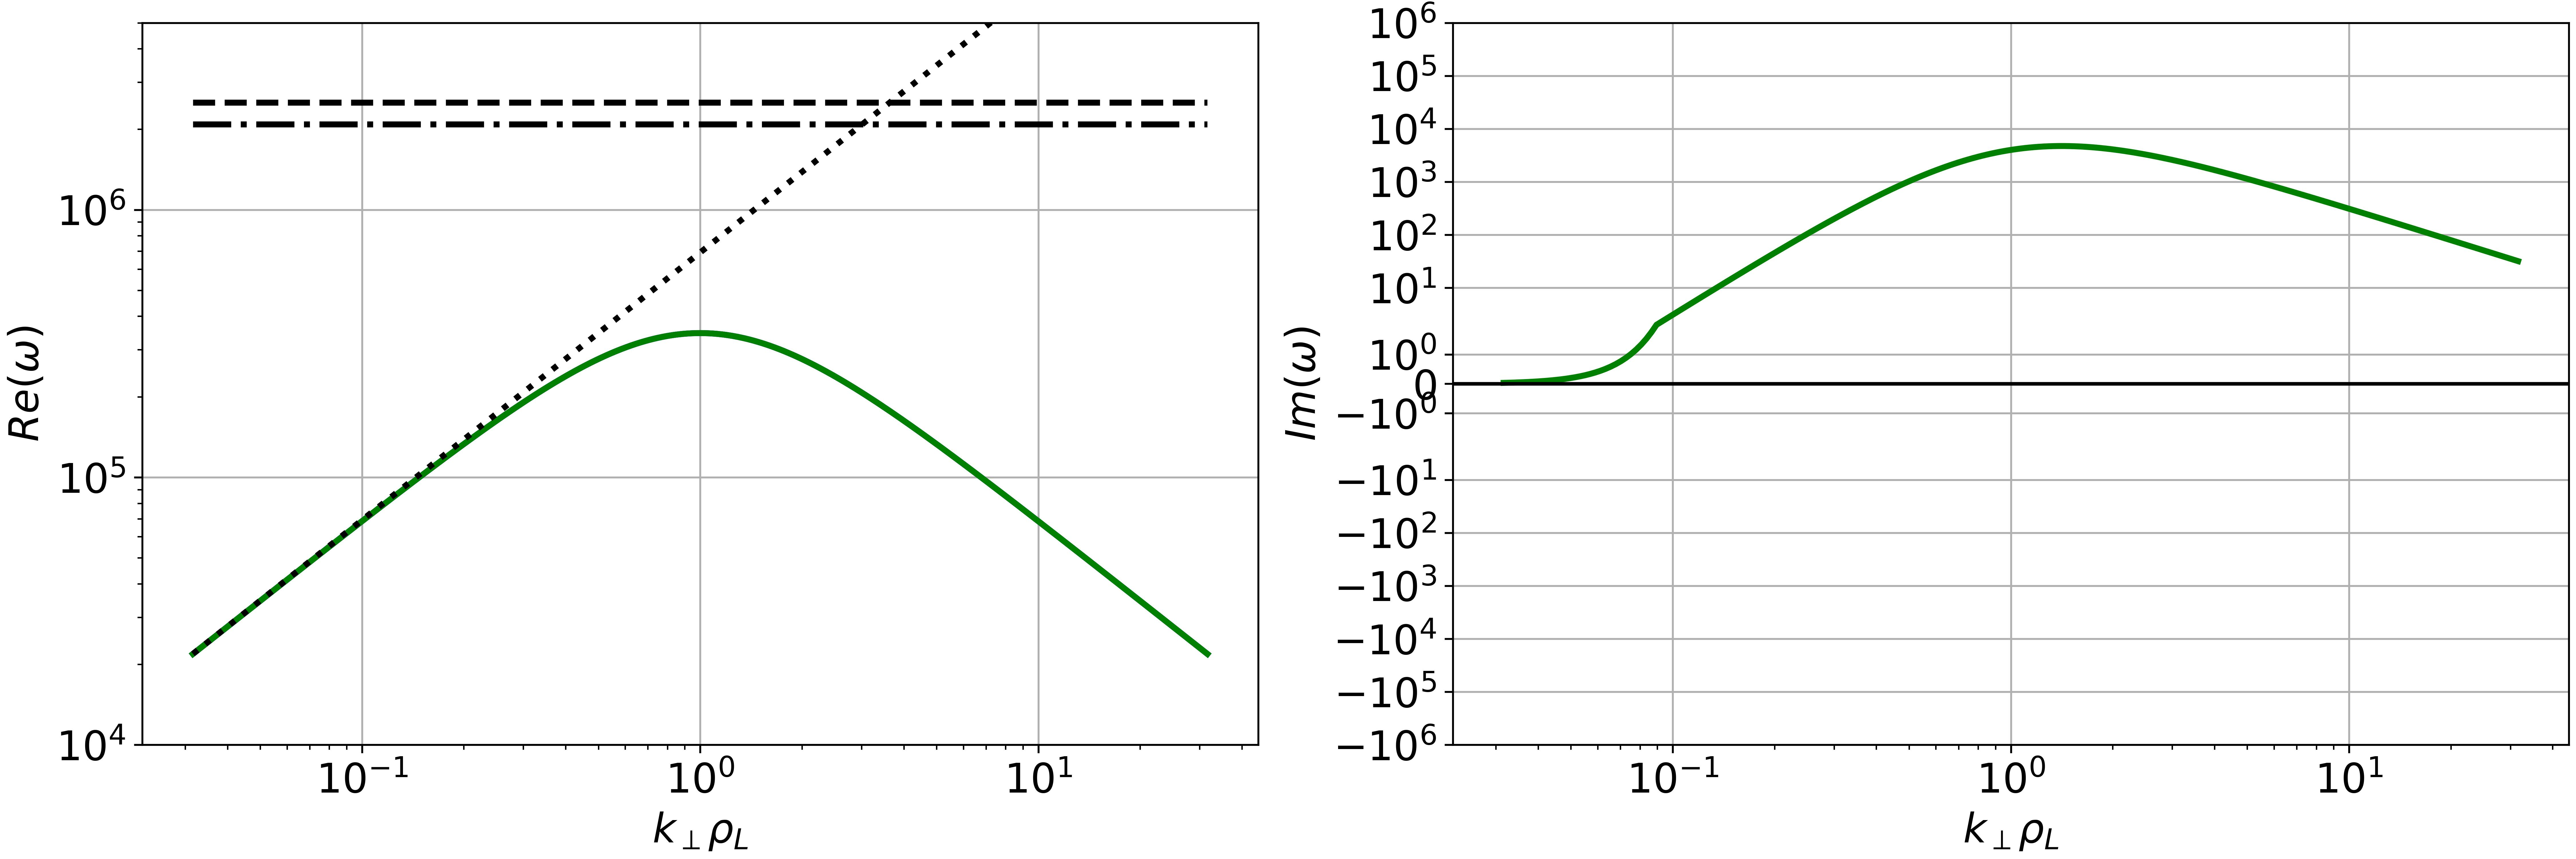
\includegraphics[width=1\textwidth]{schemes/modes_ES.jpg}
		\subcaption{Electrostatic system}
		\label{fig:edge_modesES}
	\end{subfigure}
\end{figure}
\begin{figure}[H]
	\ContinuedFloat
	\centering
	\begin{subfigure}[t]{0.85\textwidth}
		\centering
		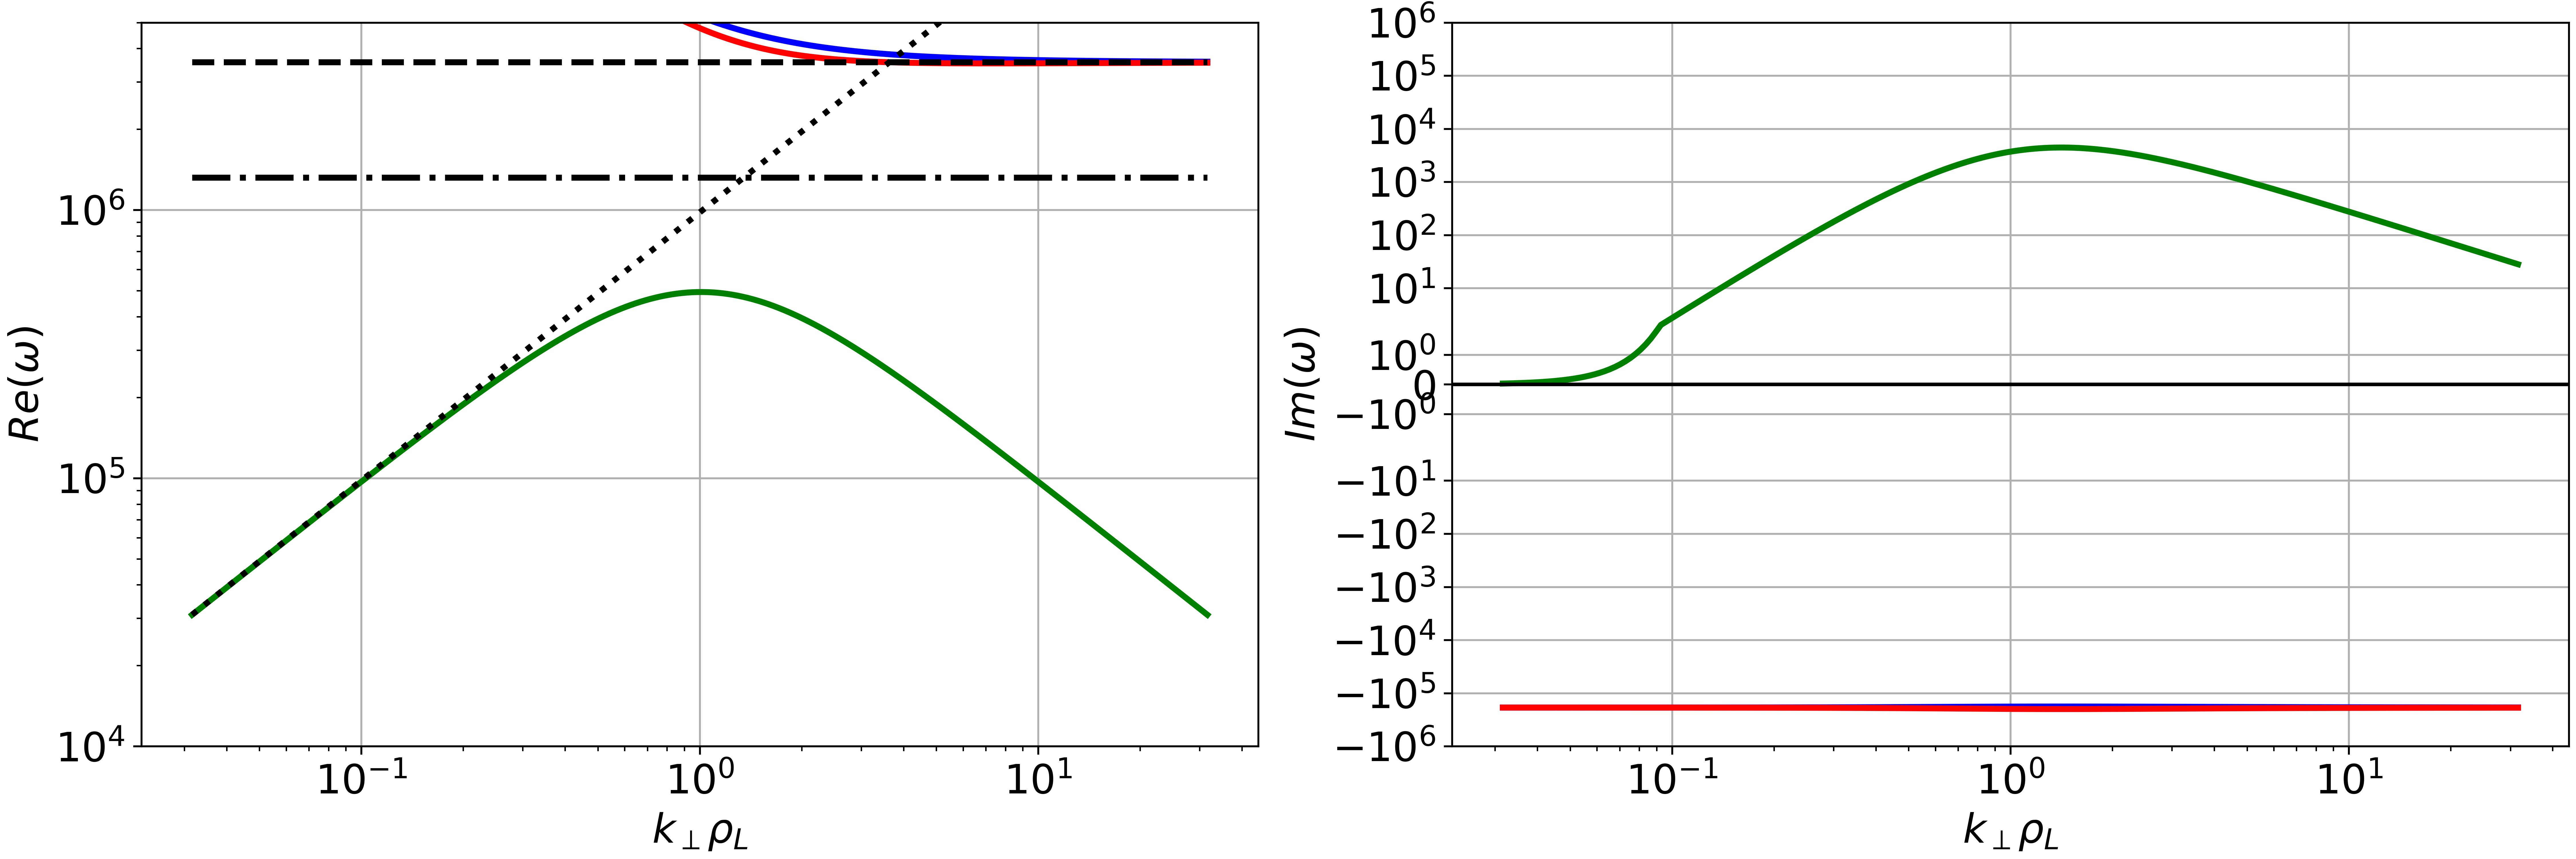
\includegraphics[width=1\textwidth]{schemes/modes_ES-inert.jpg}
		\subcaption{Electrostatic system with electron inertia}
		\label{fig:edge_modesEI}
	\end{subfigure}
\end{figure}
\begin{figure}[H]
	\ContinuedFloat
	\centering
	\begin{subfigure}[t]{0.85\textwidth}
		\centering
		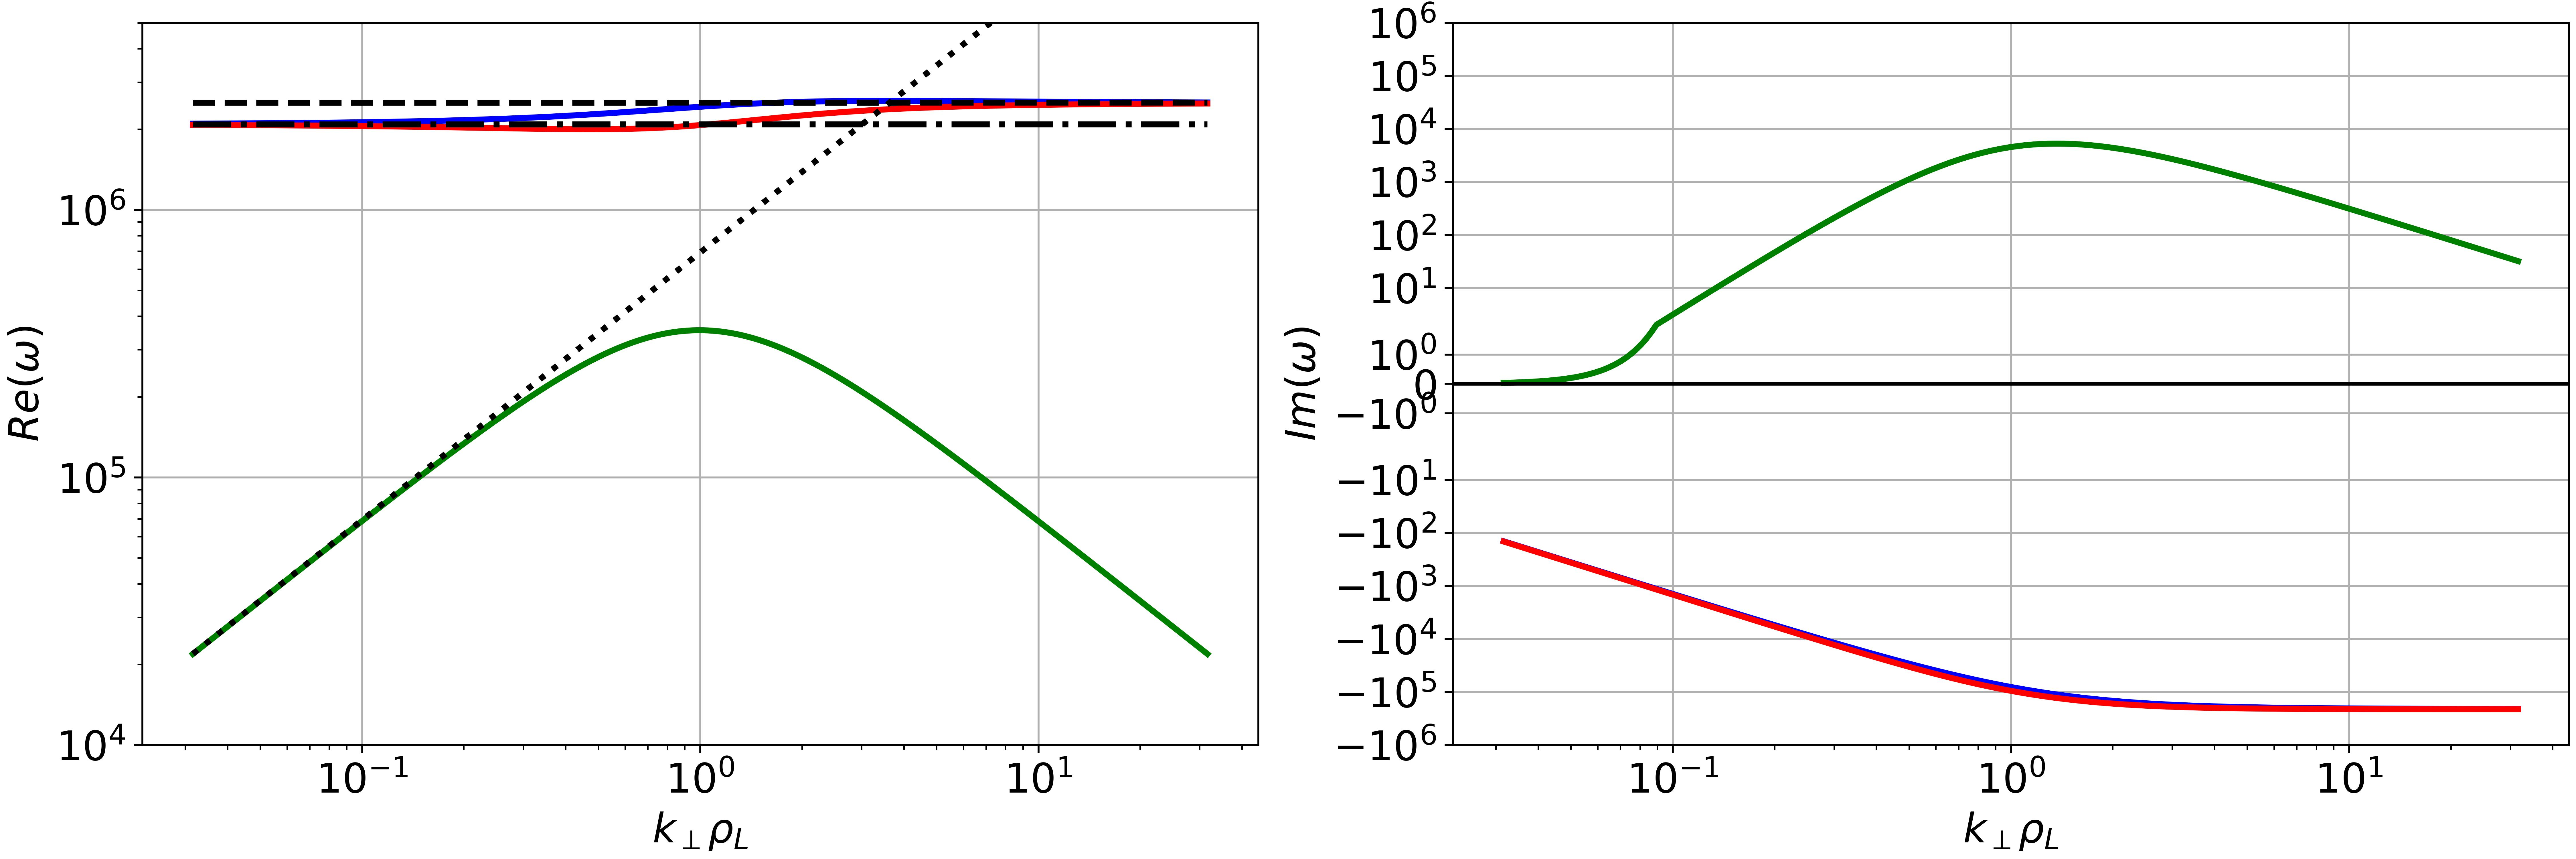
\includegraphics[width=1\textwidth]{schemes/modes_EM.jpg}
%		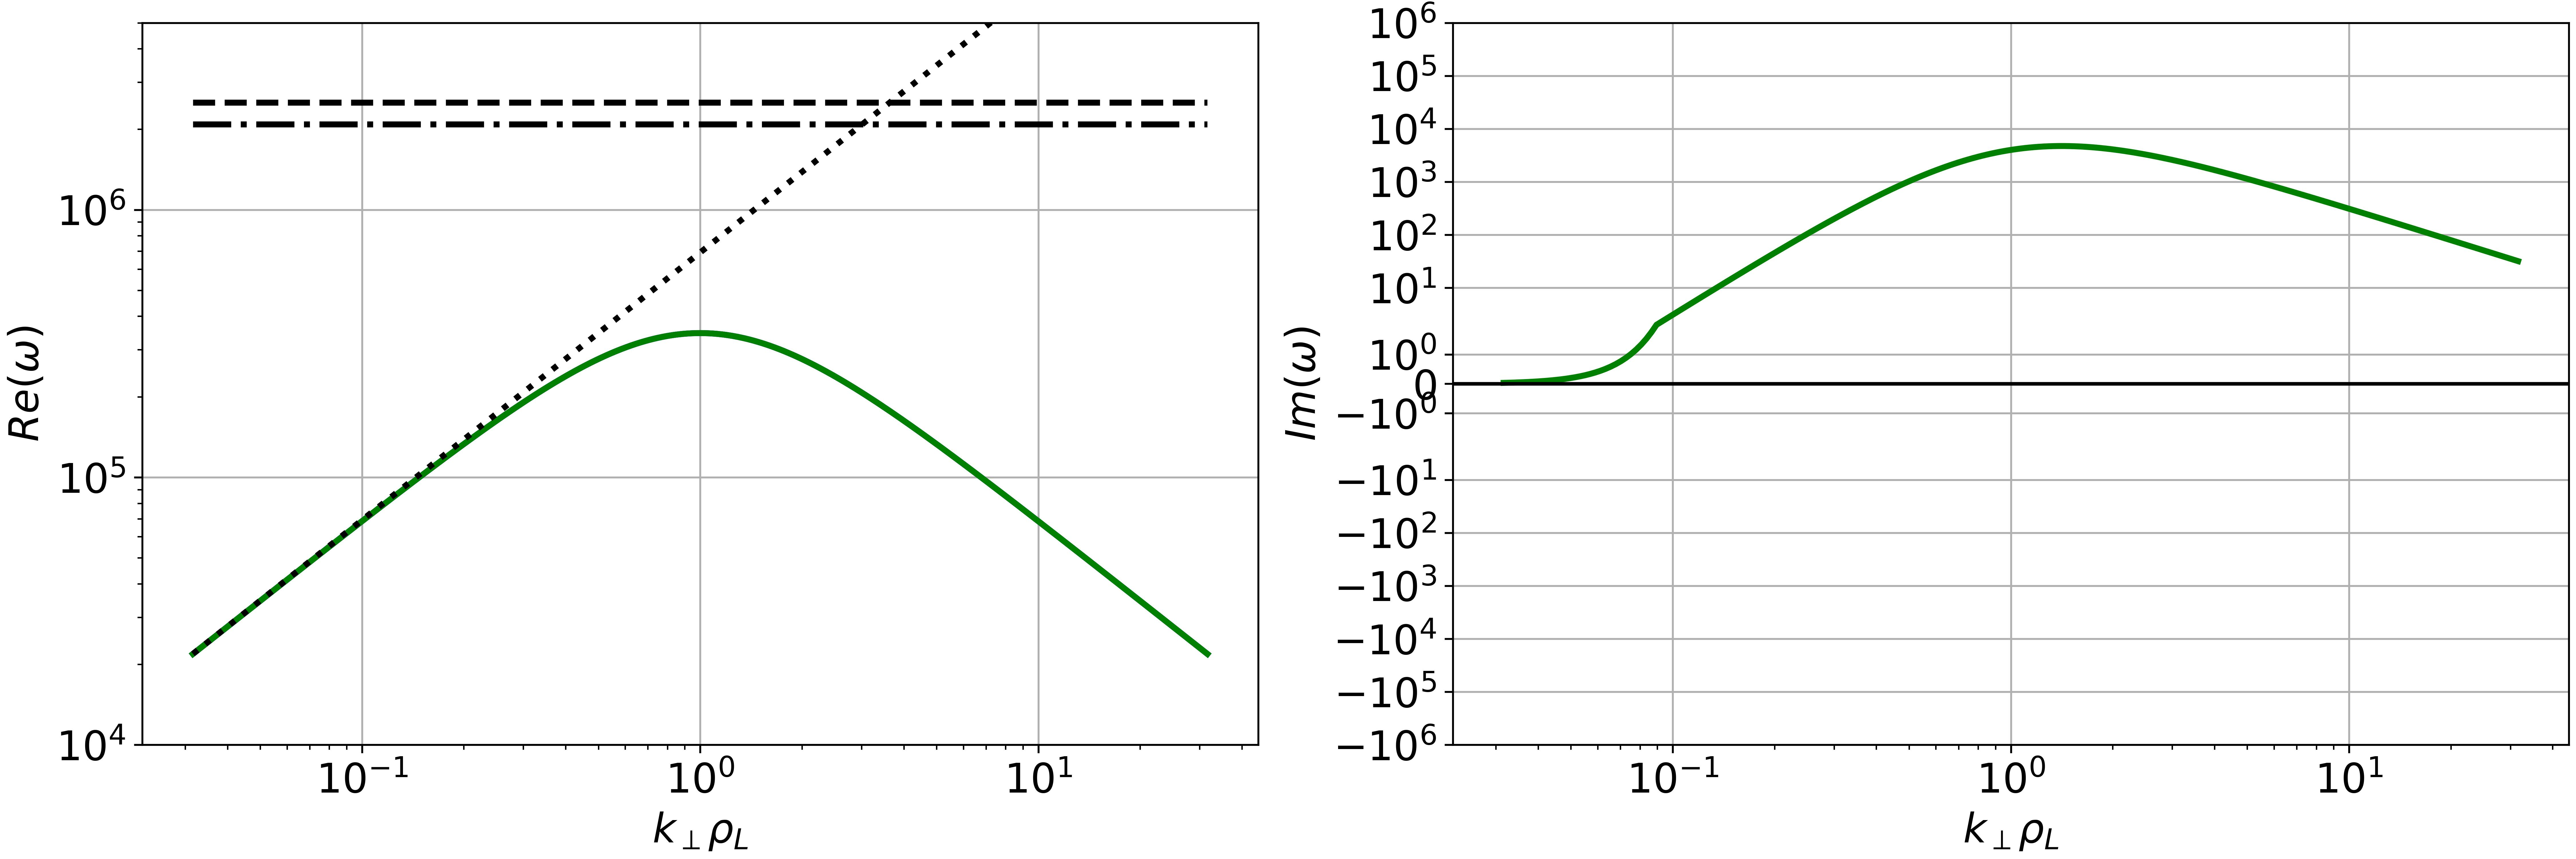
\includegraphics[width=1\textwidth]{schemes/modes_ES.jpg}
		\subcaption{Electromagnetic system}
		\label{fig:edge_modesEM}
	\end{subfigure}
\end{figure}
\begin{figure}[H]
	\ContinuedFloat
	\centering
	\begin{subfigure}[t]{0.85\textwidth}
		\centering
%		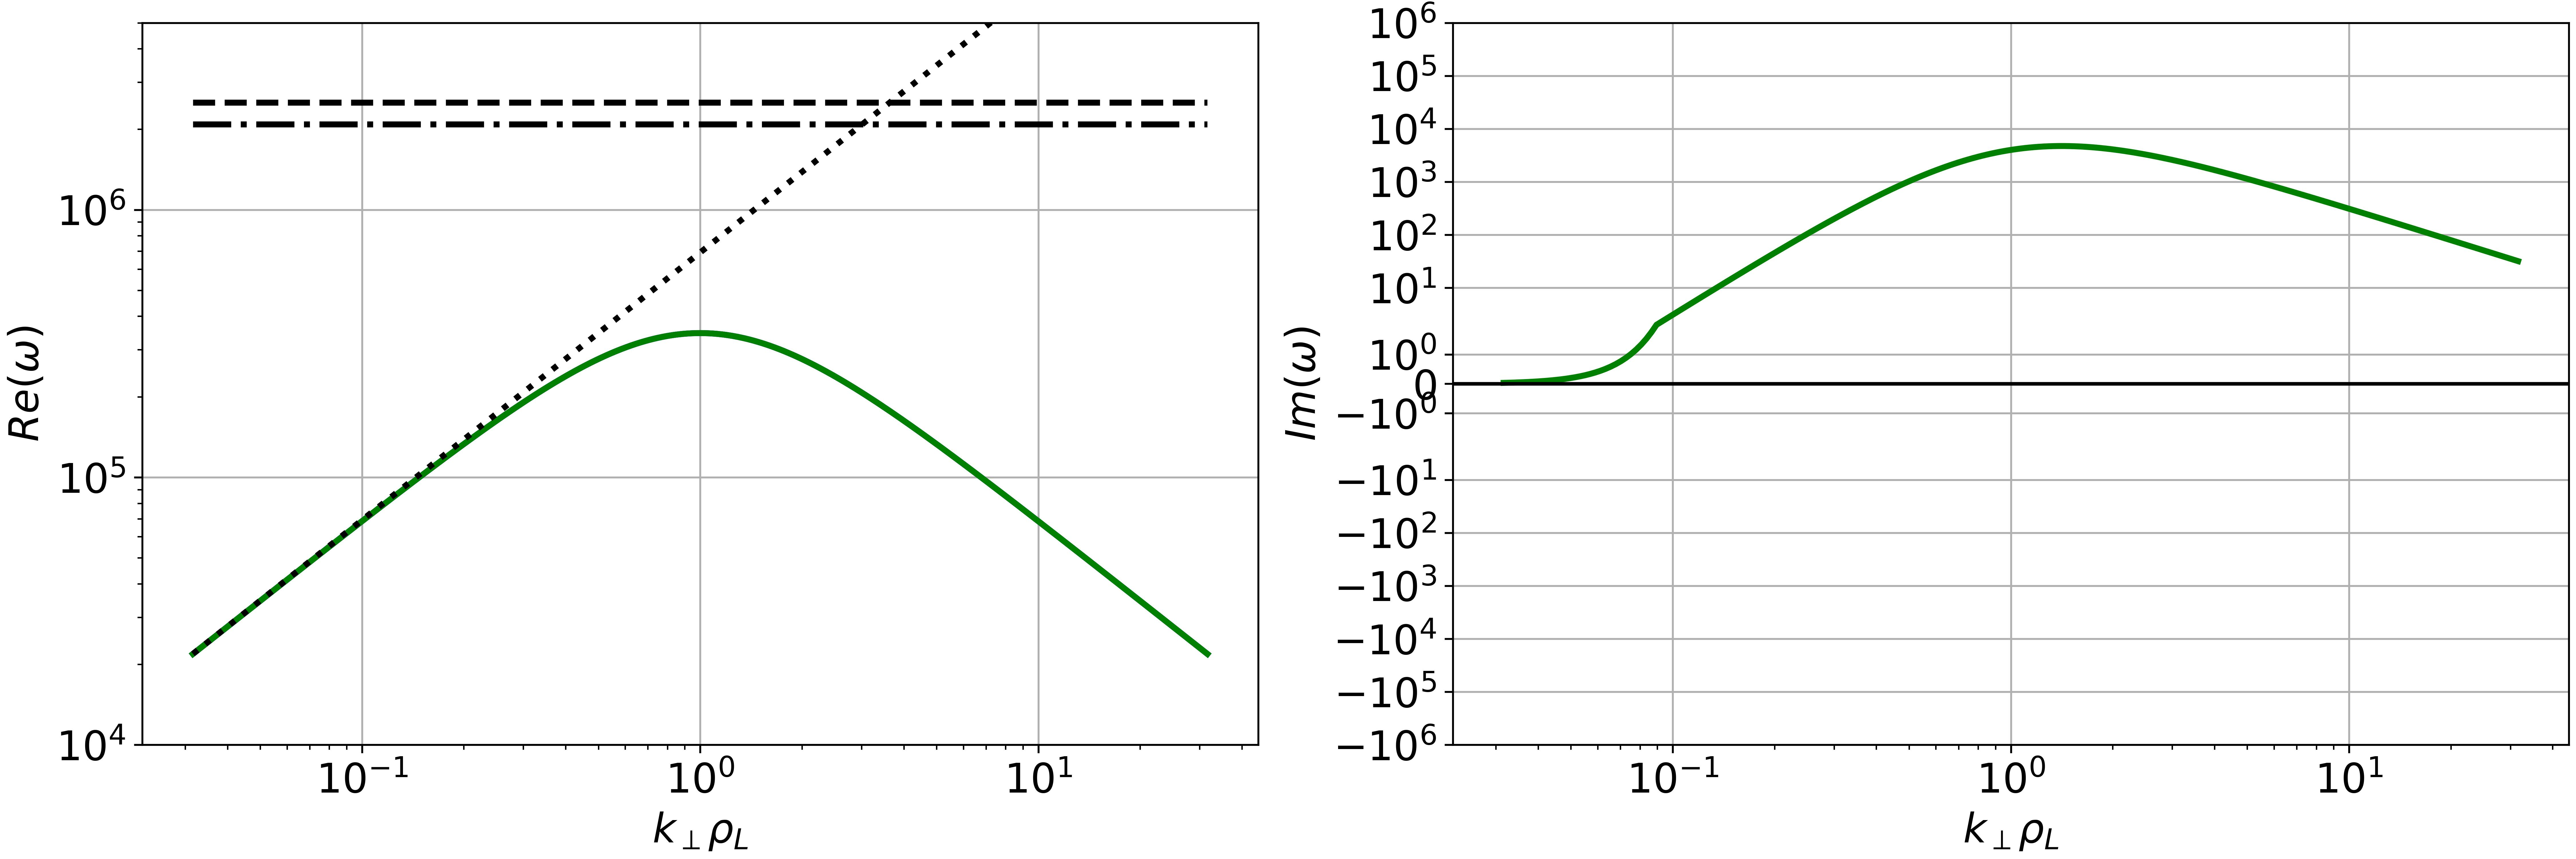
\includegraphics[width=1\textwidth]{schemes/modes_ES.jpg}
		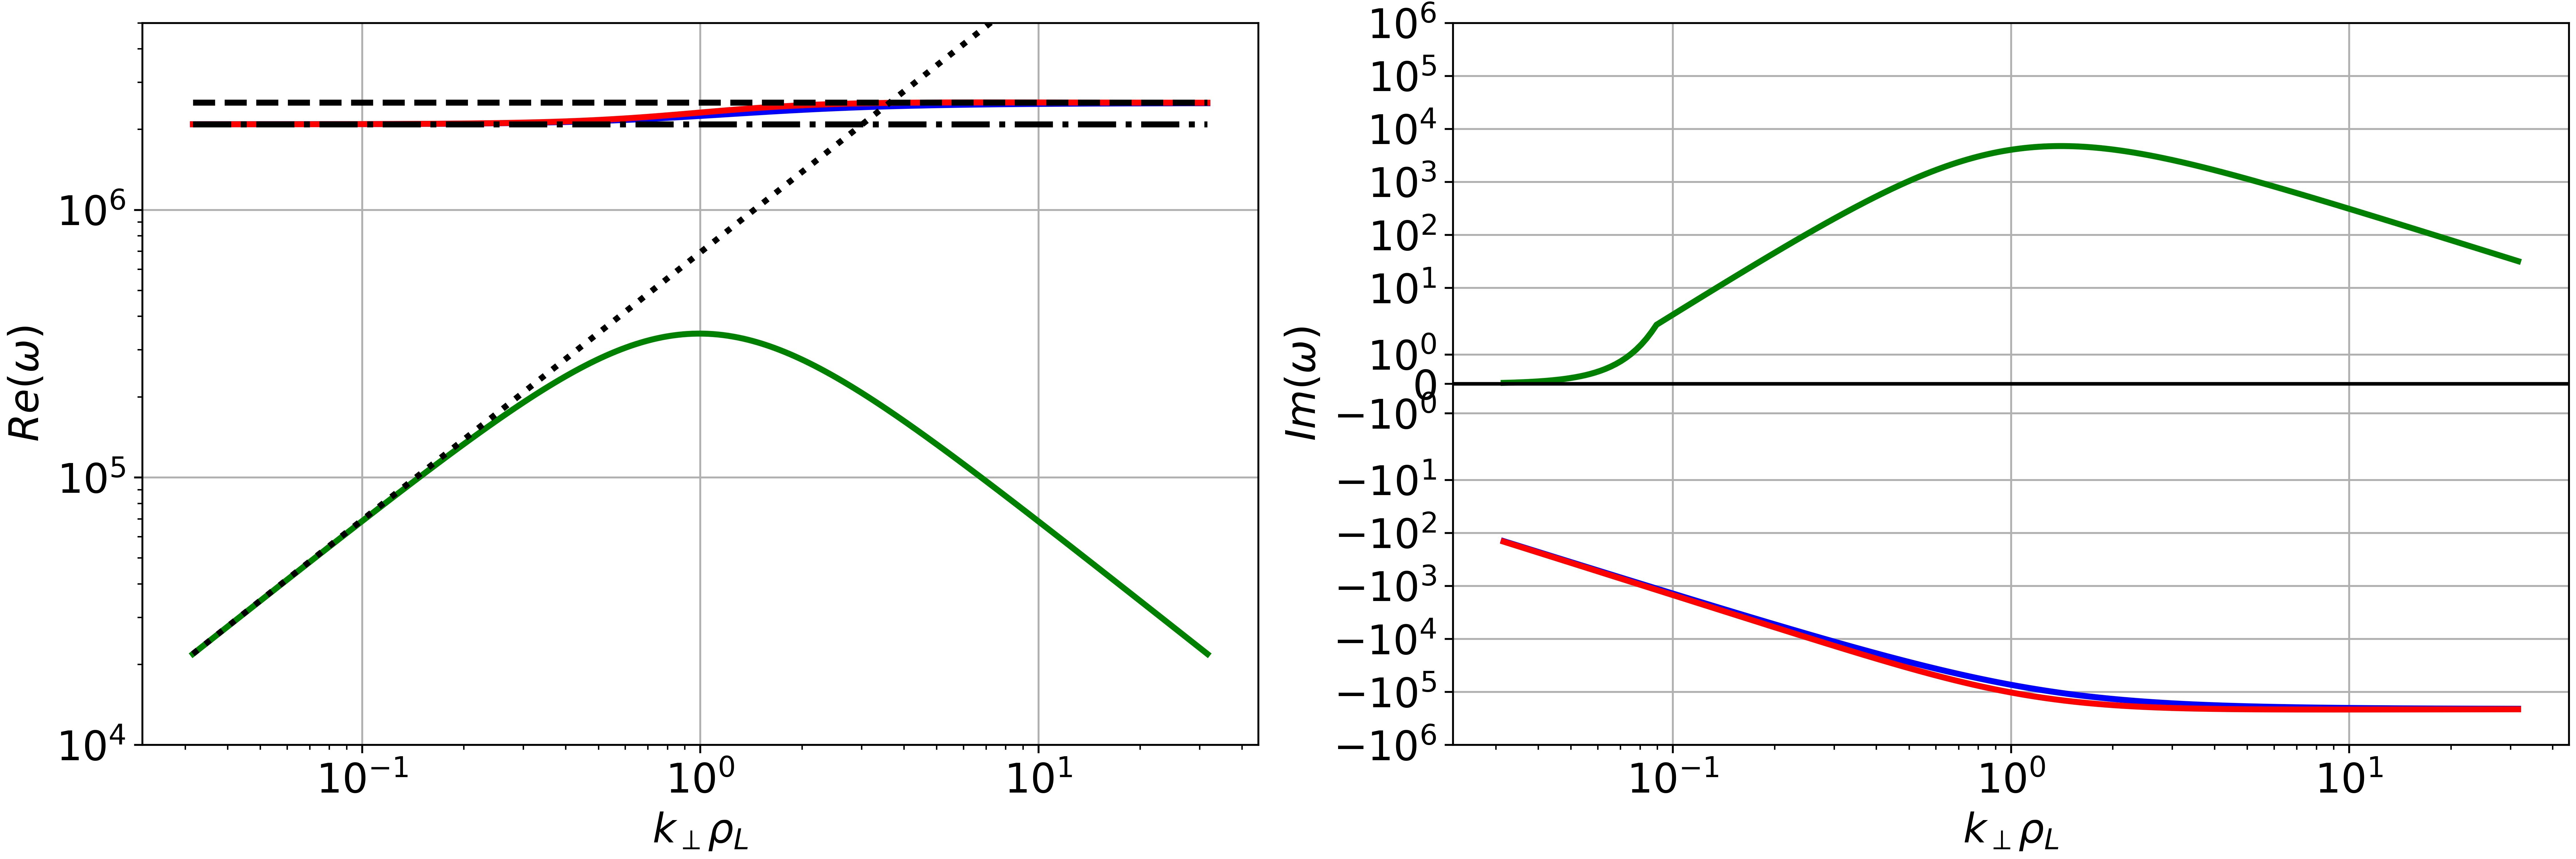
\includegraphics[width=1\textwidth]{schemes/modes_EM-flutter.jpg}
		\subcaption{Electromagnetic system with flutter}
		\label{fig:edge_modesFlutter}
	\end{subfigure}
	\caption{Dependency on the perpendicular wavenumber $k_\perp$ of the real and imaginary parts of the all solutions $\omega$ to the dispersion relation \ref{eq:edge_DAWdispersionRelation}. Except for $k_\perp$, all other values derive from: $B = 1$T, $n = 2\cdot10^{19}$m$^{-3}$, $T = 100$eV, $\lambda_p = 0.1$m and $k_\parallel = 0.6$m$^{-1}$. On a pair of graphs, a given color represents the same mode. In the left plots for $\Re{\omega}$, characteristic frequencies of the system are shown for reference ("--" diamagnetic $\omega_*$,"$\cdots$" electron sound $\omega_{s,e}$, "-$\cdot$-" Alfvén $\omega_A$).} 
	\label{fig:edge_modalBehavior}
\end{figure}

In the green curve, we observe the characteristic drift-wave frequency, which initially follows the diamagnetic frequency $\omega_*$ in the lower $k_\perp$ limit and reaches its maximum at $k_\perp \rho_L = 1$, before declining again. When the electron inertia term is introduced, a new mode emerges, starting at a significantly higher frequency before stabilizing at the electron sound frequency $\omega_{s,e} = v_{th,e} k_\parallel$. The introduction of electromagnetic terms governs the behavior of the new modes in the lower $k_\perp$ limit, which are then bounded by the shear Alfvén phase velocity. Qualitatively, the phase frequencies exhibit similar characteristics with or without flutter, with the primary difference being a more pronounced separation between the two modes as they transition from $\omega_A$ to $\omega_{s,e}$ in the pure induction. Overall, the characteristic frequencies of the electromagnetic modes are several orders of magnitude higher than the drift-wave frequency.

Looking at the growth rates associated with the modes, we first observe that drift waves are unstable with strong positive growth rates where the frequency is maximal, consistent with the earlier discussion about drift-wave instabilities. On the other hand, electromagnetic (and electron inertial) modes are very stable, showing strong negative $\gamma$. If one intends to study the growth and propagation of turbulent structures and their global impact, Alfvénic modes will only marginally contribute. It is hence possible to avoid the numerical costs involved with the high-frequency modes without much loss of accuracy.

It is more important to consider the effects of electromagnetic contributions on the drift-wave mode. For this purpose, Fig. \ref{fig:edge_comparisonDW} compares the real and imaginary parts of the drift-wave modes in the three electromagnetic scenarios with those in the electrostatic scenario.

\begin{figure}[H]
	\centering
	\begin{subfigure}[t]{0.45\textwidth}
		\centering
		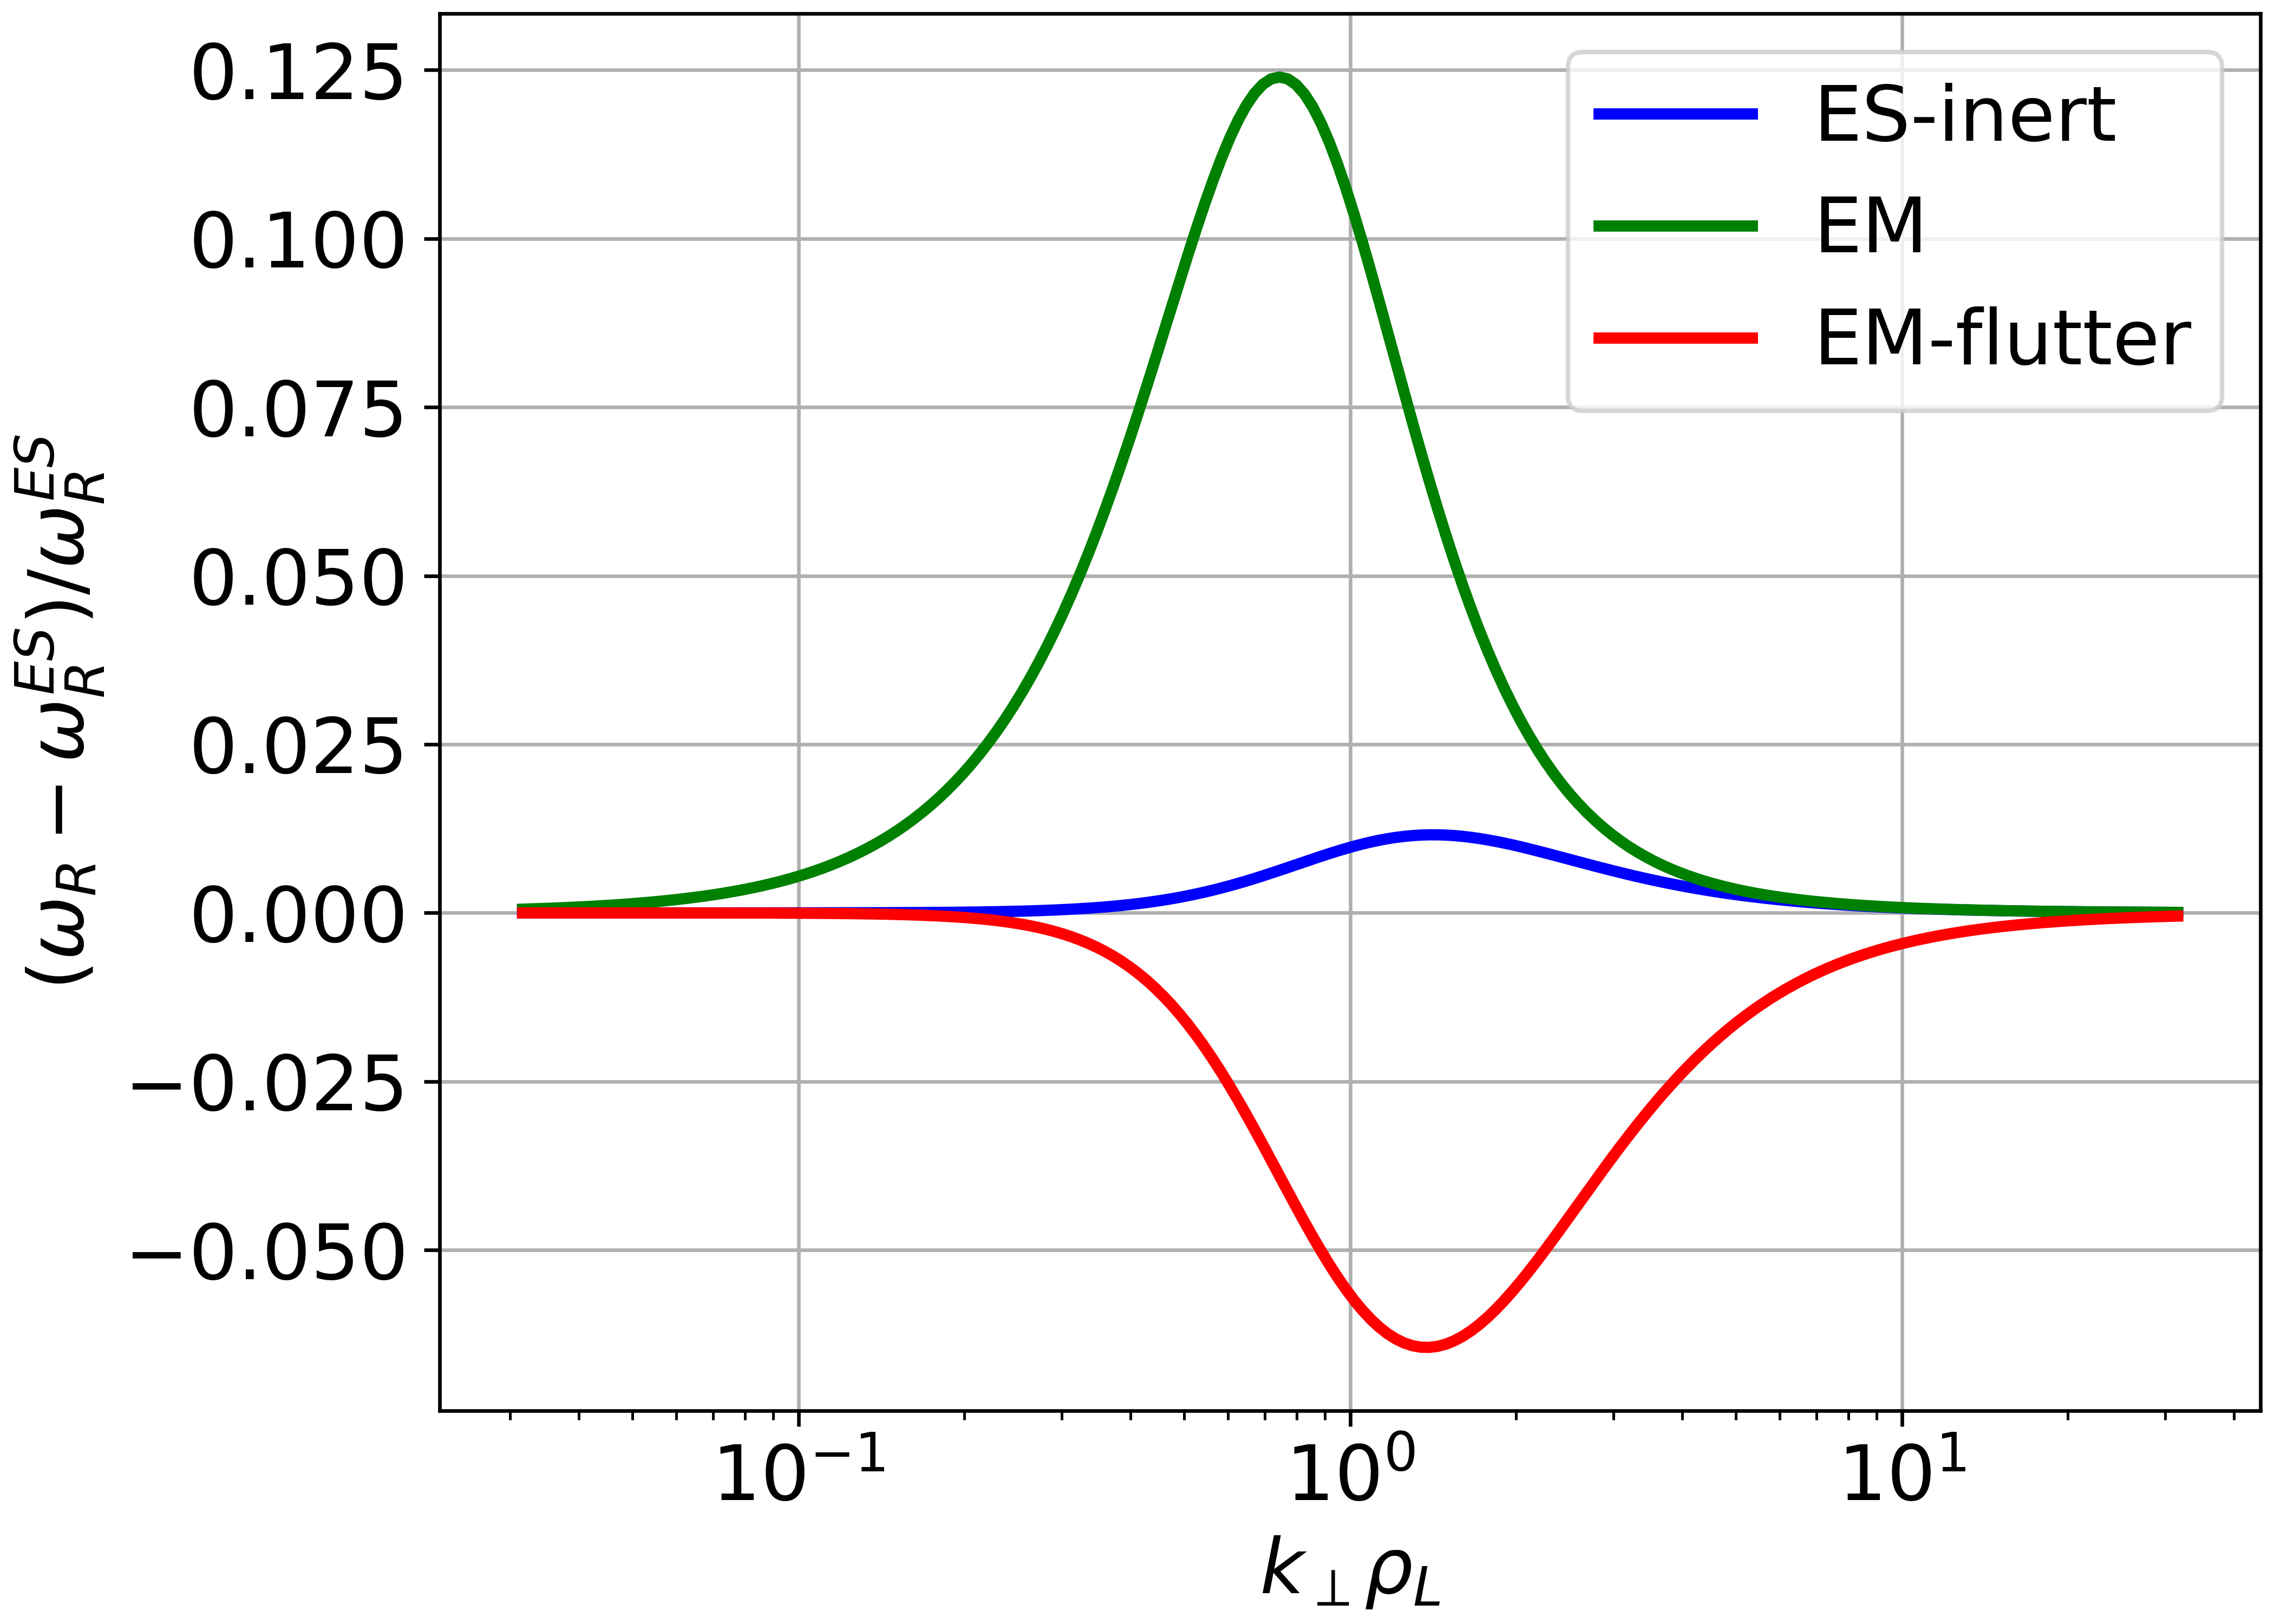
\includegraphics[width=1\textwidth]{schemes/comparison_DW_real.png}
		\subcaption{Real component}
		\label{fig:edge_comparisonDWreal}
	\end{subfigure}
	\begin{subfigure}[t]{0.45\textwidth}
		\centering
		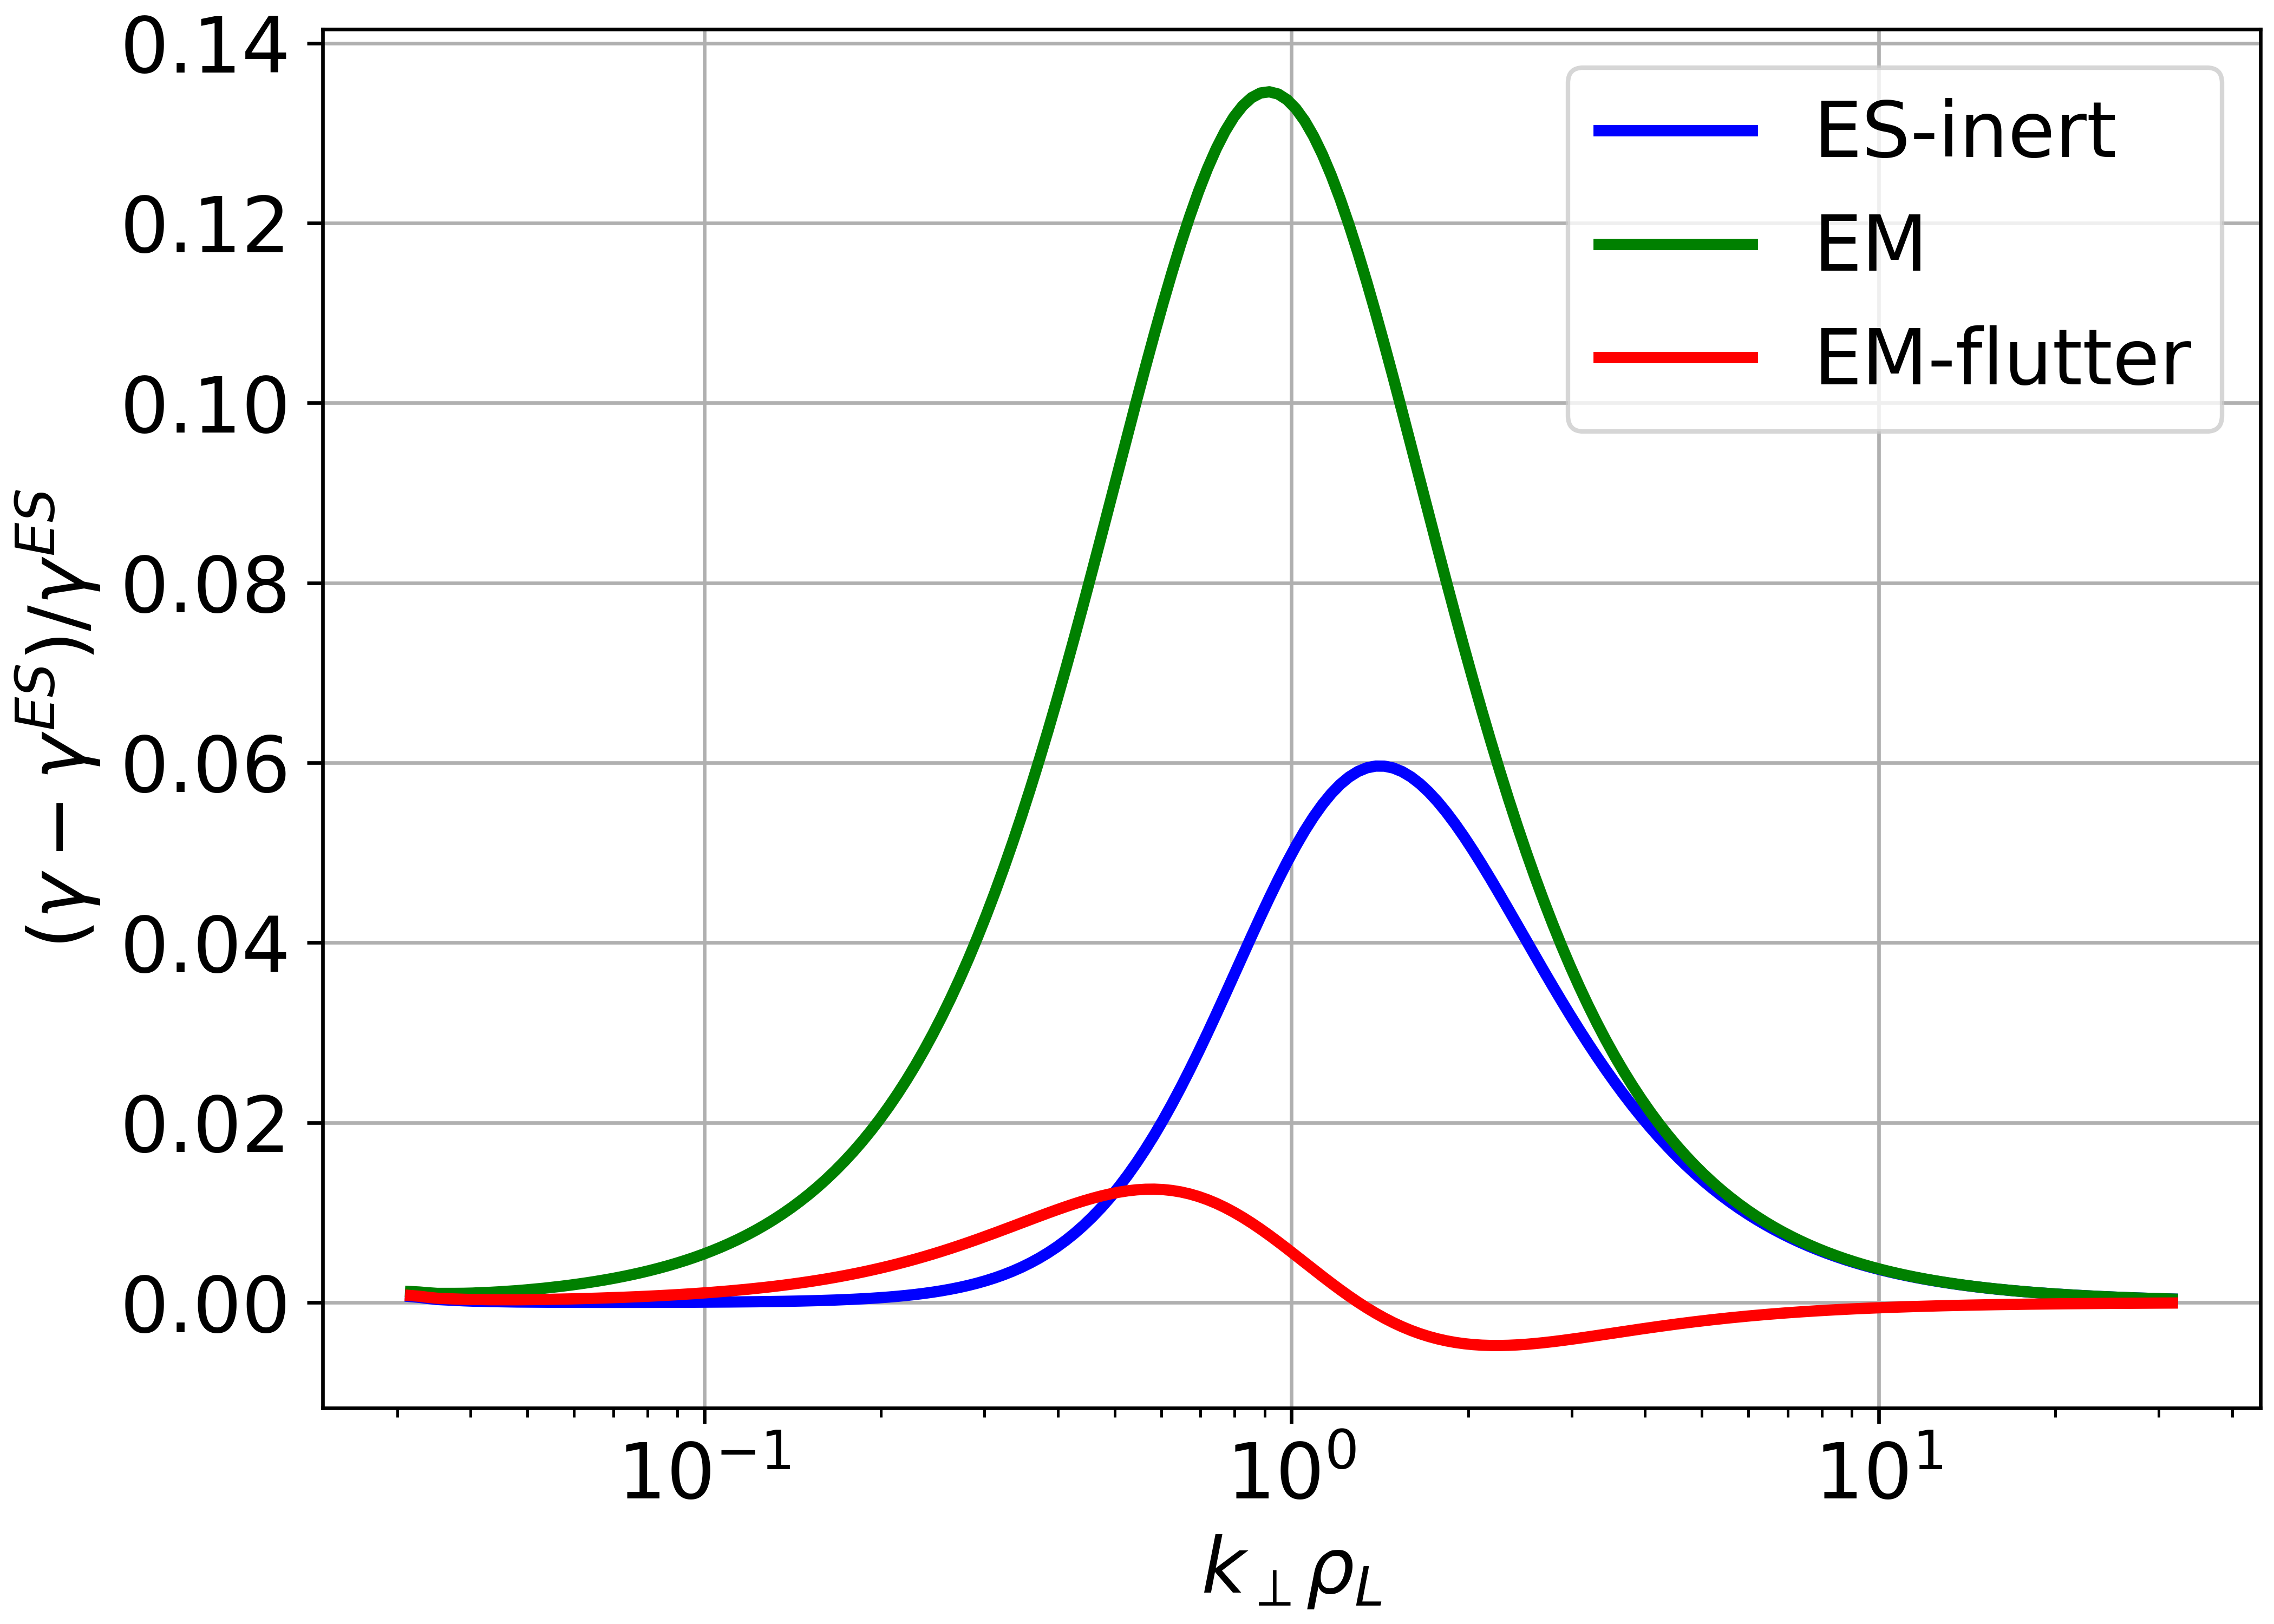
\includegraphics[width=1\textwidth]{schemes/comparison_DW_imag.png}
		\subcaption{Imaginary component}
		\label{fig:edge_comparisonDWimag}
	\end{subfigure}
	\caption{Relative difference of drift-wave frequency in the electromagnetic scenarios to the reference electrostatic case.} 
	\label{fig:edge_comparisonDW}
\end{figure}

The real part is altered by the electromagnetic additions, but the change of phase frequency will only have a minor impact on production cases. On the other hand, the growth rate increases with electron inertia and even more with electromagnetic induction. Electromagnetic flutter on the other largely mitigates the instabilities, and can even reduce the growth rate observed in electrostatic drift waves.



%\section{Electromagnetism in Other Software Projects}
%The fluid model is a somewhat popular approach to simulate transport phenomena of edge plasma and is followed by various research groups in the fusion community. Among the major actors appear the..., ..., ... . This section gives more detailed insights into the Bout++ and GRILLIX software projects, as they are both relevant for the further research done within this thesis.
%\subsection{Bout++}
%\subsection{GBS}
%\subsection{GRILLIX}
%The Max-Planck institute for plasma physics in Garching hosts the GRILLIX software project \cite{GrillixGeneralPaper} for turbulent plasma transport in the edge region on flexible 3D geometries. It distinguishes by the use of a flux-coordinate independent (FCI) approach  \cite{GrillixFCIMethod} which uses a cylindrical grid to span the tokamak. Under the assumption of a strong toroidal field it is acceptable to discretize perpendicular operators only on the Cartesian poloidal planes with typical stencils. Because the discretization is not aligned with fields or fluxes, issues with singularities along the separatrix or at the X-point are easily avoided. Parallel operators are calculated by field line tracing and subsequent interpolation which allows to use only very few poloidal planes together with a high perpendicular resolution. \\
%The Karniadakis method \cite{KarniadakisScheme} for the time advancement offers an appropriate framework to treat implicitly all terms that depend on the stiff parallel current and explicitly all other terms. At each timestep $t$, t    he following system of equation has to be solved for the density logarithm $\theta_n=\ln(n)$, the parallel ion velocity $u_\parallel$, the parallel current density $j_\parallel$ and the electric potential $\Phi$:
%\begin{equation}
%	\begin{pmatrix}
%		1 & 0 & -\frac{6}{11 n^t}\delta t \grad_\parallel  & 0 \\
%		0 & 1 & 0 & 0 \\
%		-\sigma \grad_\parallel & 0 & 1 & \sigma \grad_\parallel \\
%		0 & 0 & -\frac{6}{11}\delta t \grad_\parallel & \frac{1}{B^2}\Delta_\perp 
%	\end{pmatrix} \begin{pmatrix}
%		\theta_n^t \\ u_\parallel^t \\ j_\parallel^t \\ \Phi^t
%	\end{pmatrix} = \begin{pmatrix}
%		S_\theta \\ S_{u_\parallel} \\ 0 \\ S_\Omega
%	\end{pmatrix} \label{eq:GrillixElectrostaticImplicitSystem}
%\end{equation}
%All operators in the matrix stand for their discrete stencils, the non-linear $n^t$ is extrapolated from the three previous timesteps and the right-hand side terms $S_*$ contain the Karniadakis scheme and all explicitly solved fields. As a note, the factor $6/11$ originates in the time-stepping Karniadakis scheme. \\
%In S3X the field $j_\parallel$ in never directly computed but it is yet very present in the solved system; The gradient of the electric potential appears in the parallel Laplacian of the vorticity equation Ohm's RHS of the vorticity system with its electronic pressure and temperature gradients. The challenge of a combined parallel and perpendicular diffusion on $\Phi$, origin of the high anisotropy in S3X and main subject of this thesis, does thus not exist in GRILLIX. Further the ion density and velocity are solved explicitly in our code, so the only implicitly solved field is the electric potential $\Phi$ with its high anisotropy. \\
%In 2019, the system of equation in GRILLIX was extended by the 


